\documentclass[sigconf,anonymous,10pt]{acmart}
\usepackage{graphicx}
\usepackage{booktabs}
\usepackage{amsmath,amssymb}
\usepackage{subcaption}
\usepackage{tikz}
\usepackage{soul} % enables \hl{} — highlights detector-correction edits for review

\usetikzlibrary{arrows.meta, positioning}
\graphicspath{{figures/}}

%% Conference info — update when you have the official details from AINTEC
\acmConference[AINTEC '26]{Proceedings of the 21st Asian Internet Engineering Conference}{December 1--3, 2026}{Taipei, Taiwan}
\acmYear{2026}
\copyrightyear{2026}
\acmArticleSeq{8}
\begin{document}

\title{The Local Path Not Taken: Traffic Tromboning and Routing Inefficiency in Pakistan}

%% Authors are anonymised for double-blind review.
%% Remove the anonymous block and add real author info for camera-ready.
\author{Anonymous Author(s)}
\affiliation{%
  \institution{Anonymous Institution}
}
\email{anonymous@example.com}

\renewcommand{\shortauthors}{Anonymous et al.}

\begin{abstract}
% Efficient and reliable Internet access is of utmost importance during both normal network conditions and faults such as submarine cable interruptions. 
Despite being connected to multiple submarine and terrestrial Internet cables, Pakistan's Internet connectivity is far from ideal. With a concerted push towards online service delivery and economy digitization, the robustness of the local Internet connectivity becomes key. We use 14 RIPE Atlas probes on the last-mile, connected to 9 different ISPs in 7 Pakistani cities in a week-long experiment, capturing 305,116 ping and 200,292 traceroute measurements. Measurements are made to 98 websites that form a stratified proportional sample of the most popular content accessed from Pakistan across different sections of the critical infrastructure hosted by Pakistani operators, CDNs, and offshore operators.  

For sites hosted by Pakistani operators domestically, we find that almost 6\% of accesses involve path tromboning, with the rate of tromboning varying by ISP, and type of content. The financial sector was the worst off, with 55\% of accesses tromboning. We did not find any evidence of data that traversed any of the four Pakistani Internet eXchange Points (IXPs). Some ISPs privately peer with CDN operators, without peering with each other. As a result, access to CDN-hosted sites content is upto 12 times slower for other ISPs compared to the one privately peering with the CDN host. We estimate that access to content hosted domestically can be significantly faster and more robust if IXPs are better utilized through multi-faceted incentive mechanisms. 

% Pakistan operates an Internet exchange, PKIX, in three cities with dozens of connected member
% networks, yet in a week of hop-level measurement not one of 222,944 traceroutes to Pakistani
% destinations crossed its peering fabric: the exchange is built but, for most traffic, not used.
% We measure the consequence from inside the country. From every RIPE Atlas probe connected in Pakistan we run TCP traceroutes
% and pings to a fixed, reproducibly sampled set of 100 Pakistani websites---stratified across
% critical-infrastructure sectors and across local, CDN, and offshore hosting---once an hour and once
% every half hour for a week, and we classify each path as domestic or hairpinned using a detector
% grounded in round-trip-time physics rather than unreliable IP geolocation. The uniform, longitudinal design
% lets us report, on equal terms and per ISP, how much domestic traffic trombones abroad and through
% which transit operators, what latency this costs and whether the cost is structural or diurnal,
% and---from routing verdicts that flip between local and hairpinned across the week---whether a
% domestic path exists for the traffic that nonetheless leaves the country. Over 204,384 analysed
% traceroutes we find that international paths never exceed $10\times$ the speed-of-light floor
% while 24\% of domestic paths do; that 15.1\% of traces to Pakistani-hosted sites leave the
% country and return (3--31\% by source ISP, and 86\% for state banking sites); that the same
% anycast content is a median $12.7\times$ slower on the worst-peered major ISP than on the best;
% that the penalty is structural, varying under 3 percentage points across the day; and that 83\%
% of the probe--site pairs that ever hairpin are also served domestically on other rounds of the
% same week---direct evidence that the local path exists and is not taken. The finding of the study is
% that the local path exists but is not taken, and that PKIX is the instrument that would take it.
\end{abstract}

%%


%%
\begin{CCSXML}
<ccs2012>
<concept>
<concept_id>10003033.10003079.10011704</concept_id>
<concept_desc>Networks~Network measurement</concept_desc>
<concept_significance>500</concept_significance>
</concept>
<concept>
<concept_id>10003033.10003083.10003090.10003091</concept_id>
<concept_desc>Networks~Topology analysis and generation</concept_desc>
<concept_significance>300</concept_significance>
</concept>
<concept>
<concept_id>10003033.10003039.10003045.10003046</concept_id>
<concept_desc>Networks~Routing protocols</concept_desc>
<concept_significance>100</concept_significance>
</concept>
</ccs2012>
\end{CCSXML}

\ccsdesc[500]{Networks~Network measurement}
\ccsdesc[300]{Networks~Topology analysis and generation}
\ccsdesc[100]{Networks~Routing protocols}

\keywords{Internet exchange points, traffic tromboning, Pakistan, hairpinning, developing regions, PKIX, RIPE Atlas, latency, routing measurement}
\acmArticleSeq{8}
\maketitle


\section{Introduction}
Pakistan has over 150 million broadband internet users served mostly over seven submarine cables~\cite{pta2026telecom}. Pakistan's Internet gets disrupted frequently by submarine cable faults. In 2022 alone, %there
six such faults were reported~\cite{opalinski2024quest}. 

Nearly 37\% of the 0.2M most popular domains in Pakistan are either hosted by local network operators or by international CDN operators that also have local caches in Pakistani ISP networks~\cite{tranco}. Content hosted within Pakistan should be available even in the face of submarine cable faults. Furthermore, under normal network operation, the locally hosted content should be available at low latencies, and low packet loss, irrespective of the user's ISP. To achieve this, local network and hosting providers must peer with each other. 

Private peering solves this issue, but requires $O(n^2)$ peering sessions, where $n$ is the number of network and hosting providers. This puts a strain on the routers and the interconnection network. An Internet Exchange Point (IXP) provides a shared physical location where many operators can peer at once through a route server. CDN operators also prefer IXPS over private peering to place their caches~\cite{opalinski2024quest}. This results in lowered latency and packet loss to CDN-hosted content in addition to that hosted by local operators.

Multiple studies have measured the extent of paths to local content tromboning through international transit providers and found gaps in the effectiveness of IXPs in developing countries~\cite{gupta2014, edmundson2016characterizing, obriain2017rebuilding}. For such countries, effective local peering is important also because path tromboning results in unnecessary international transit fees straining already scarce foreign exchange reserves. 

%It was empirically shown that peering at an IXP in Italy resulted in lower and more stable latency~\cite{ixp-worth-peering}. Lui observed that while having more internet bandwidth through submarine cables helps, having an effective IXP can reduce average latencies by upto $64$\% in the Pacific island countries of Fiji, Samoa, and New Zealand~\cite{lui2021costings}.

There are four IXP sites across Pakistan, three sites under the umbrella of PKIX established in 2017, and one named PIE powered by DE-CIX, established in 2024. Together, these IXPs have dozens of participants. 
%When one of them accesses any service hosted in Pakistan, whether it is hosted by a Pakistani organization, or a CDN cache located in Pakistan, the traffic should remain within Pakistan. Yet, often such traffic is routed back through offshore routers (path tromboning) or the content is served from offshore CDN caches. This has three distinct costs: elevated latency, cost of international transit bandwidth, and unnecessary risk exposure in the face of submarine cable faults. %This is not a failure of infrastructure in the conventional sense. Pakistan operates two internet exchanges, PKIX in three cities and PIE in Karachi, with dozens of participating operators. The physical remedy exists, yet for most Pakistani internet traffic, it is not being used.
%
%The problem has a specific structure. Four operators have international gateway infrastructure in Pakistan: PTCL, Transworld, Cybernet and the Special Communications Organization (SCO)\cite{pacra2026telecom}. The latter's retail footprint is confined to Azad Jammu \& Kashmir and Gilgit-Baltistan rather than the broader national market. %, so its gateway capacity is the least utilized of the four. 
%Figure~\ref{fig:gateway-capacity} shows installed versus activated capacity across the four operators. PTCL's AA-1 alone accounts for the largest single share, while Cybernet's PEACE cable and SCO's overland OFC link are the least utilised, at 38\% and 20\% activated respectively.
% Effectively, PTCL, Transworld, and Cybernet serve not only as international bandwidth providers to smaller ISPs, but also as transit providers between them. This should work fine in principle, however, in practice, it does not. % the same destination can be reached one way or another depending on the path: a Worldcall address we measured separately is local ($\sim$46\,ms) through PTCL but trombones through Singapore ($\sim$134\,ms) through Transworld, even though both operators serve the same country. A local path exists; it is simply not always the one used. When traffic instead leaves the country and comes back before reaching its destination, we call it traffic tromboning. This has two distinct costs: elevated latency during ordinary operation, and elevated exposure during submarine-cable faults, when internationally-routed traffic significantly degrades.
%
% \begin{figure}[t]
%   \centering
%   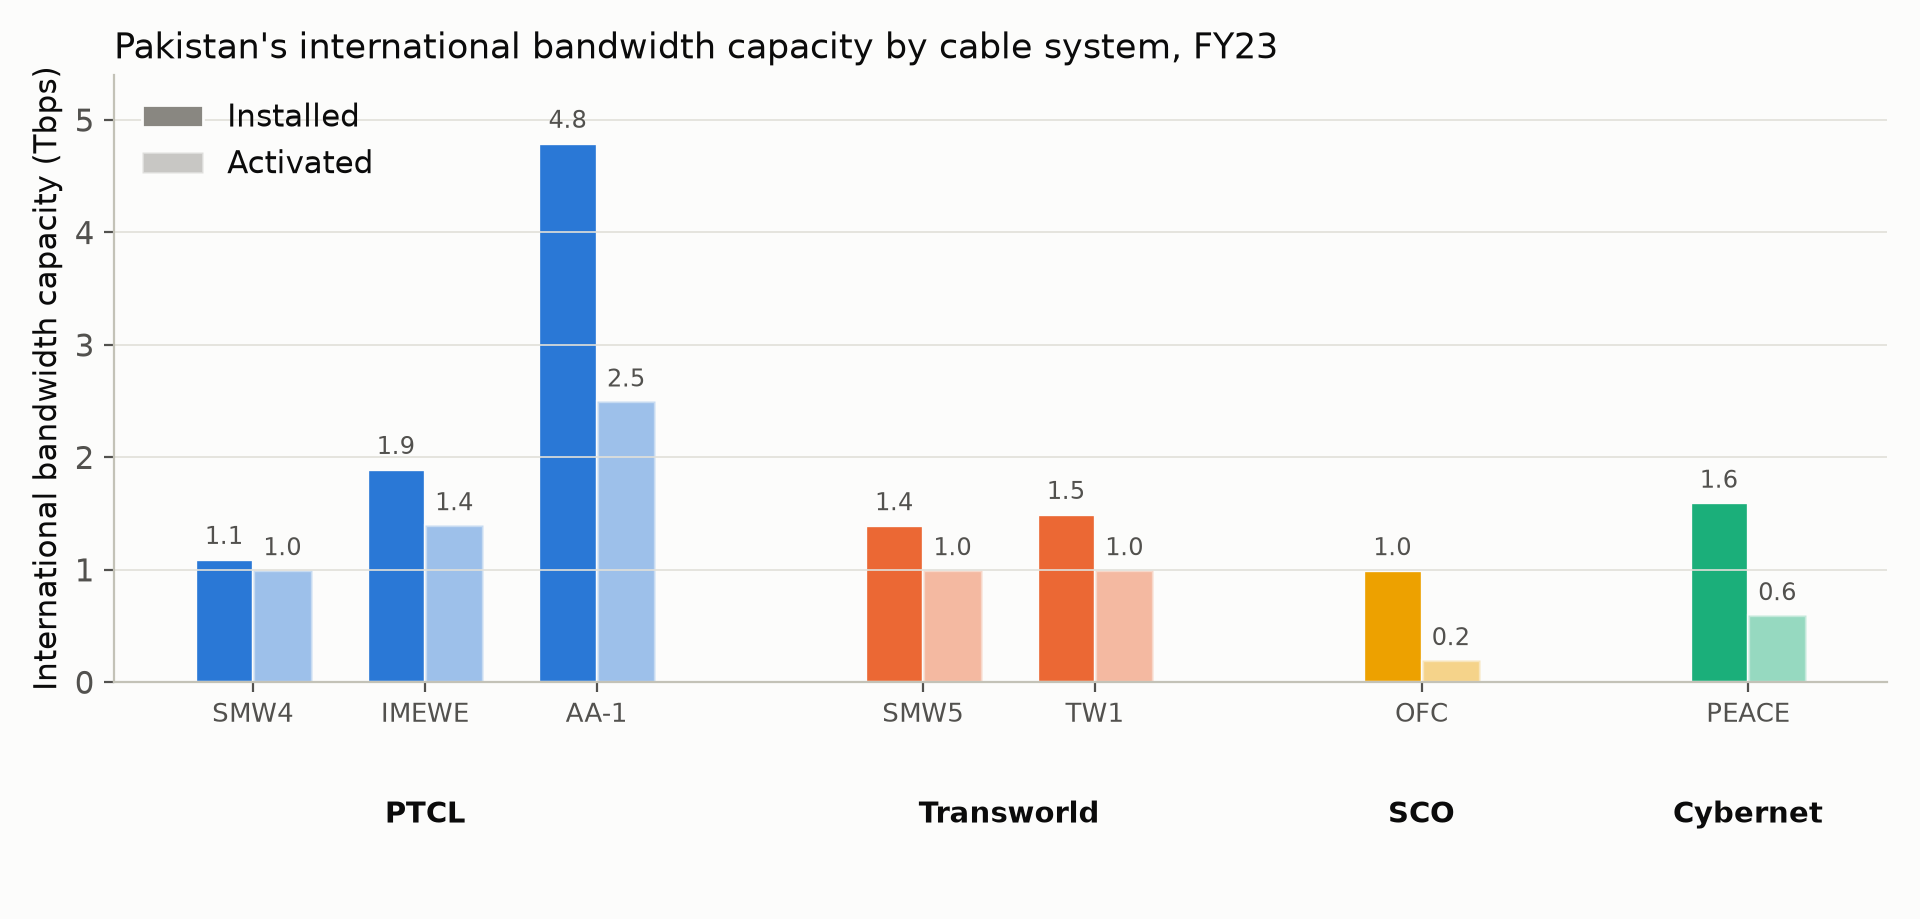
\includegraphics[width=\columnwidth]{fig_gateway_capacity.png}
%   \caption{Pakistan's international bandwidth capacity by cable system and operator, FY23. Recreated from PACRA data~\cite{pacra2026telecom}, coloured by gateway operator.}
%   \label{fig:gateway-capacity}
% \end{figure}
%
%
%
%Private peerings can alleviate tromboning, but require $O(n^2)$ peering sessions where $n$ is the number of ISPs. An internet exchange point (IXP) provides a shared physical location where many networks can peer at once through an IXP route server. %, avoiding the need for each pair to arrange a separate connection. Without peering at such an exchange, two ISPs in the same city will still route traffic through one of the three international gateway operators: PTCL, Transworld, or Cybernet.
%
%Pakistan operates two internet exchanges, PKIX in three cities and PIE in Karachi, with dozens of participating operators. The physical remedy exists, yet for most Pakistani internet traffic, it is not being used.
%
%PKIX's own published figures show inter-ISP latency dropping from 100--144\,ms internationally to 1--31\,ms through the exchange~\cite{pta2026}, 
PKIX claims that inter-ISP latencies have dropped from more than 100\,ms (routed internationally) to less than 50\,ms (routed through the exchange)~\cite{pta2026}. %Independent verification of PKIX's effectiveness is largely unexplored. 

Establishing an IXP is not merely a technical exercise, it requires the willingness of the competing stakeholders to cooperate and connect their traffic. Therefore, it is important to determine the effectiveness of the Pakistani IXPs using a diverse set of neutral vantage points.

%Across a week of hop-level measurement from inside Pakistan, we could not find evidence of any of the 222,944 traceroutes to Pakistani hosted destinations crossing the IXP peering fabrics.


%In this paper
To bridge this gap, we use active measurements from $14$ RIPE Atlas probes distributed across Pakistani ISPs to measure the effectiveness of the IXPs. We run traceroutes and pings over a week-long window to $98$ websites spanning government, education, banking, news, and other sectors. %and we classify each path using an RTT-physics detector that does not rely on IP geolocation. Our three research questions are:
Using this dataset, in this paper, we aim to answer the following three research questions:

\begin{description}
  \item[RQ1] To what extent does Pakistani internet traffic trombone through foreign networks, and which ISPs and transit paths are responsible?
  \item[RQ2] What is the quantifiable RTT cost of tromboning, and is this penalty stable over time or does it vary with time of day or day of week?
  \item[RQ3] For destinations that trombone, does a local path demonstrably exist? 
  \item[RQ4] Do users of different ISPs in the same city get a similar latency to a locally hosted site?
  %, evidenced by routing verdicts that flip between local and hairpinned across the measurement window?
\end{description}

While answering these questions, we make the following contributions:
\begin{itemize}
    \item Deployment of a geo-diverse set of RIPE Atlas public probes in %far flung 
    rural and urban areas of Pakistan, providing a rare end-user view of the Internet experience from different parts of the country. These probes are also placed in different ISPs' networks. This enables not only the analysis presented in this paper, but also serves as a testbed for future studies by other researchers.
    %\item The above probes also differ by the serving ISPs, providing a rich testbed for future researchers.
    \item We make the first-ever week-long trace of ping and traceroute data, and associated code, between 14 probes and 98 target sites, spanning Pakistani-, CDN-, and internationally-hosted services, available to the community for further investigation.
    %\item We make available the code that may be used to analyze these and other similar traces by the research community.
\end{itemize}

Our findings show that IXP is largely under-utilized. In most cases a local path already exists but is not chosen. We also find that the resulting excessive latency penalty is unevenly distributed across ISPs. %The central argument of this paper is simple: Pakistan does not need to build new infrastructure to improve its internet routing. Incentives are needed to broaden participation at the IXP to include CDN operators and smaller ISPs, and activate local traffic exchange at the IXP.

\section{Related Work}
\label{sec:related-work}
This section describes related work in the context 
of usefulness of local peering 
delivering a measurable latency benefit in mature markets
(\S\ref{subsec:rw-value}), followed by highlighting failures of 
local peering in developing -world (\S\ref{subsec:rw-underuse}). 
We then describe Pakistan's physical topology
and transit market characteristics within that literature (\S\ref{subsec:rw-market}), and close
by showing that Pakistan's physical topology compounds the market-structure
problem and that no prior study has tested it directly, which motivates the
present work (\S\ref{subsec:rw-topology}).

\begin{comment}
% This long comment encloses last version of Related Work. 
% Whole section is kept as it is because there are some major 
%structural changes in the section.
% Including: Combining last two sub-sections and adjusting 
% intro to the section accordingly.   
\section{Related Work}
\label{sec:related-work}

This section makes our case in four steps. We first show that local peering
delivers a measurable latency benefit in mature markets
(\S\ref{subsec:rw-value}). We then show that developing-world exchanges
systematically fail to deliver that benefit, for two distinct and
independent reasons: underused peering, and offshore hosting that peering
alone cannot fix (\S\ref{subsec:rw-underuse}). We then situate Pakistan's
transit market within that literature (\S\ref{subsec:rw-market}), and close
by showing that Pakistan's physical topology compounds the market-structure
problem and that no prior study has tested it directly, which motivates the
present work (\S\ref{subsec:rw-topology}).

\subsection{Local Peering}
\label{subsec:rw-value}
The value of local peering in developed markets is well established, and
treated primarily as a question of latency optimization. IXP paths for
Italian ISPs deliver both lower and more stable latency than upstream
transit, avoiding a detour through an intermediate network
abroad~\cite{dibartolomeo2015}. This matters at scale too: large exchanges
such as DE-CIX and AMS-IX carry a substantial share of European and Asian
interdomain traffic~\cite{ager2012, chatzis2013}. A similar active,
end-to-end approach has already been used in our own region: SLAC's PingER
framework, a network of distributed monitoring agents that ping and
traceroute a fixed set of remote hosts, benchmarked South Asian countries
against the developed world~\cite{ali2017internet}. We adopt the Italian
study's vantage-point design, national probes measuring national targets,
and its framing of locality as a form of network sovereignty, but replace
its hand-picked target list with a complete, reproducibly sampled candidate
pool of Pakistani websites (\S\ref{subsec:sites}).

\subsection{Peering Underuse and Hosting Geography in the Developing World}
\label{subsec:rw-underuse}
In developing countries, local peering matters not only for latency but
because path tromboning leaves the local network exposed whenever an
international transit cable faults. IXPs across the developing world sit
under-utilized for two distinct reasons, both of which we also observe in
Pakistan: local ISPs are frequently absent from their national IXP
altogether, or physically present but never establishing bilateral peering
sessions with one another. In Africa this leaves $66.8$\% of interdomain
paths between residential networks and local Google cache infrastructure
detouring through Europe before returning to a destination that was never
far away, and correcting it would compress intra-continental latency to a
floor of roughly $30$~ms~\cite{gupta2014}, a number that echoes PKIX's own
published figures of $1$ to $31$~ms through the exchange against $100$ to
$144$~ms for the international alternative~\cite{pta2026}. The same
underlying dependence can be measured directly at a country level:
extending global AS customer-cone and hegemony metrics to a
country-specific version shows exactly how concentrated a country's
Internet is on a small number of, often foreign, autonomous
systems~\cite{huffaker2023asrank}.

Peering alone is not enough: it cannot fix tromboning where the underlying
content is not domestically hosted at all. More than half of Brazil's and
Kenya's most popular domestic websites resolve to servers in the United
States or United Kingdom, and roughly $13$\% and $50$\% of measured paths
in these countries, respectively, trombone as a direct
consequence~\cite{edmundson2016characterizing}. This motivates us to
include CDN-hosted as well as locally hosted sites in our measurement. The
same asymmetry shows up in government hosting specifically: across 61
countries, governments deliver 62\% of URLs from third-party infrastructure
overall, but the regional split is wide, 68\% of government bytes in North
America against just 5\% in South Asia, so for a government site the
hosting decision itself, not only its ISP's peering, decides whether a
citizen's traffic ever needs to leave the country~\cite{kumar2024govhosting}.

Underuse is not fixed destiny; it responds to deliberate investment rather
than merely to an exchange's existence. Uganda's national IXP grew from
$3$ participants in $2001$ to only $24$ by $2017$, until a switching-fabric
upgrade and the onboarding of Akamai's CDN pushed peak traffic from
roughly $300$~Mb/s to over $2$~Gb/s within a single
year~\cite{obriain2017rebuilding}. A similar pattern holds in the South
Pacific, where weighted average latency for Pacific island nations fell by
$64$\% once a hybrid IXP was established~\cite{lui2021costings}.

\subsection{Pakistan's Transit Market Structure}
\label{subsec:rw-market}
Pakistan is not land-locked like Uganda, so its tromboning sits closer to a
hosting- and peering-driven account than to a pure geographic-isolation
problem. That points to market structure rather than physical isolation,
and treating it as a pure engineering problem risks understating why it
persists. Three operators, PTCL, Transworld, and, more recently, Cybernet,
hold the only licensed international gateways, and every other domestic
ISP buys upstream connectivity from one of them~\cite{pacra2026telecom}. As
we confirm in \S\ref{sec:rq1}, these same three operators perform nearly
all of the hairpin hand-offs we observe. Whether that concentration is the
reason these ISPs have little incentive to peer with one another is a
claim our routing data alone cannot test, but it is consistent with the
pricing record: PTCL's partial $2006$ privatization did not produce a
decline in wholesale gateway pricing in the years that followed, unlike
the mobile network sector in the same country~\cite{gonzalez2026peering}.
This asymmetry matches the broader soft-budget-constraint literature:
incumbents facing limited competition have little incentive to pass
through efficiency gains, regardless of the physical capacity or
infrastructure already available to them.

\subsection{Topology }
\label{subsec:rw-topology}
Pakistan's international connectivity is concentrated almost entirely at a
small number of Karachi landing stations operated by the same limited set
of gateway licensees, while cross-border terrestrial alternatives remain
commercially unused for reasons of state security policy rather than
engineering cost~\cite{opalinski2024quest}. The routing patterns we
measure are governed by this same physical topology and the same small set
of gateway operators.

The closest prior Pakistan-focused measurement work found that Pakistan's
traffic to its own South Asian neighbors, India, Bangladesh, and Bhutan
among them, routes through Europe or Singapore rather than
directly~\cite{ali2017internet}. That is the same detour pathology we
study, but observed between countries rather than within one, and measured
with an aggregate ping benchmark rather than a per-ISP, per-hop
attribution. No prior work has tested whether this same failure occurs
domestically inside Pakistan, or whether Pakistan's own IXPs are actually
used once traffic never needs to leave the country. That is the gap this
paper closes.
\end{comment}

% \section{Background}

% The value of local peering is well established in developed markets, where it is
% treated primarily as a question of latency optimization.
% Di Bartolomeo et al.~\cite{dibartolomeo2015} compare IXP versus upstream transit
% paths for Italian ISPs %using RIPE Atlas measurements combined with controlled BGP announcements, 
% and find that IXP paths deliver both lower and more stable latency
% while %preserving traffic locality, that is,  keeping domestic traffic on domestic infrastructure rather than 
% avoiding routing domestic traffic through an intermediate network abroad. Large-IXP studies of mature exchanges such as DE-CIX and AMS-IX~\cite{ager2012,
% chatzis2013} motivate why this matters at scale. %: peering density at a handful of major European and Asian exchanges is treated as a settled proxy for a healthy, cost-efficient domestic internet. 
% Our study borrows Di Bartolomeo et al.'s
% vantage-point design (national probes measuring national targets) and their framing
% of locality as a form of network sovereignty, but departs from their hand-picked
% target list in favor of a complete, reproducibly sampled candidate pool of Pakistani
% websites (\S\ref{subsec:sites}). % We also observe that IP geolocation is unreliable, and augment it with a locator grounded in RTT physics.

% %This same failure mode, an exchange point that exists but is not used to capacity, recurs whenever the literature turns to the developing world, suggesting it is structural rather than incidental. 
% In developing countries, local peering is important not only for latency optimization, but also critical due to commonplace path tromboning. Faults on an international transit cable often partition even the local network. Multiple studies have found under-utilized IXPs in developing countries. Gupta et al.~\cite{gupta2014} measure interdomain paths between residential access networks and local Google cache
% infrastructure in Africa and find that $66.8$\% of these paths %leave the continent entirely, 
% detour through Europe before returning to a destination that was never far away. They attribute this to two distinct failures that we also observe in Pakistan. First, local ISPs are frequently completely absent from their national IXP. Second, even ISPs that are physically present at the exchange frequently fail to establish bilateral peering sessions with one another. Gupta et al. estimate that correcting for these would result in compressing African intra-continental latency
% to a floor of roughly $30$~ms. This number echoes PKIX's own published figures of $1$ to $31$~ms through the exchange against $100$ to $144$~ms for the international
% alternative~\cite{pta2026}.

% Edmundson et al.~\cite{edmundson2016characterizing}
% show that peering infrastructure alone cannot fix tromboning where the underlying content is not domestically hosted at all. They found that more than half of Brazil's and Kenya's most popular domestic websites resolve to servers in the United States or United Kingdom. They also found that roughly $13$\% and $50$\% of measured paths in these countries, respectively, trombone %through those jurisdictions 
% as a direct consequence. %a hosting-driven detour that persists regardless of local IXP investment. 
% This motivates us to include CDN-hosted as well as local hosted sites in our measurement study.
% %our own three-way hosting classification (\S 3.1): a domestic exchange only resolves tromboning for traffic that is domestically hosted to begin with, and our finding that CDN-fronted Pakistani sites are tromboned in a bimodal, all-or-nothing pattern (\S 4.2) is consistent with their account of hosting geography, not peering alone, as a binding constraint.

% \'{O} Briain et al.~\cite{obriain2017rebuilding} observe that the national IXP in Uganda increased
% from $3$ participants in $2001$ to only $24$ by $2017$. Then, a switching-fabric upgrade and the onboarding of Akamai's CDN acted as a catalyst and pushed peak traffic from roughly $300$~Mb/s to over $2$~Gb/s within a single year. This shows  that underuse responds directly to deliberate investment, not merely the exchange's existence. Similarly, Lui~\cite{lui2021costings} documents %an equivalent pattern in the South Pacific: island nations already connected to New Zealand via submarine cable still see a weighted average latency of 44.21~ms absent a functioning subregional exchange, 
% weighted average latency for South Pacific island nations falling by $64$\% %, to 15.99~ms, 
% once a hybrid IXP was established. %model coordinates traffic properly. %Lui's central finding is methodological rather than technical, since co-locating hardware at a shared facility does not by itself produce peering.

% %Unlike Uganda's landlocked dependence on a small number of submarine cable landings abroad,
% %Pakistan has direct coastal access via Karachi, so the mechanism producing
% Pakistan isn't land-locked like Uganda, so the tromboning here sits closer to Gupta et al.'s and Edmundson et al.'s hosting- and
% peering-driven accounts. %than to a pure geographic-isolation problem.
% That gap is not solely a lack of coordination between the ISPs and CDNs, and treating it as a pure
% engineering problem risks understating why it persists. The ISPs appear not to have an incentive to peer due to the international gateway market being a legal triopoly: only PTCL, Transworld, and, more recently, Cybernet hold international gateway licenses. Every other domestic ISP purchases upstream connectivity
% from one of them~\cite{pacra2026telecom}. Gonzalez~\cite{gonzalez2026peering}
% observes how PTCL's partial $2006$ privatization %, a 26\% stake sold to Etisalat,
% did not produce a decline in wholesale gateway pricing in the years that followed,
% %in sharp contrast to Pakistan's mobile retail sector, where genuine competitive
% unlike the mobile network sector in the same country. %entry by Telenor, Jazz, and Zong over the same period drove rapid price declines.
% This asymmetry is consistent with the broader soft-budget-constraint literature:
% incumbents facing limited competition %competitive discipline at the specific market layer that
% % matters have correspondingly 
% have limited incentive to pass through efficiency gains,
% regardless of the physical capacity or infrastructure already available to them.

% Opalinski et al., work on documenting Pakistan's physical
% layer~\cite{opalinski2024quest}, %extend this account and show it is not confined to commercial
% %incentives alone: 
% showing that Pakistan's international connectivity is concentrated almost entirely at a small number of
% Karachi landing stations operated by a limited number of %the same two 
% gateway licensees, while
% cross-border terrestrial alternatives %, despite Pakistan sharing borders with India,
% %Afghanistan, and Iran, 
% remain commercially unused for reasons of state security policy rather than engineering cost. %; a Lahore to Amritsar terrestrial fiber link,
% %commissioned in 2008, has to date never carried commercial traffic. 
% The routing patterns we measure are governed by the same underlying physical topology and the small set of gateway-operators.

% %Finally, our measurement design itself builds on established active-measurement practice. We combine RIPE Atlas~\cite{ripeatlas} as our active-measurement platform, RIPEstat~\cite{ripestat} for prefix and routing metadata, and Team Cymru bulk WHOIS with an RDAP fallback for ASN and registry resolution where WHOIS data is stale or unavailable.

\section{Methodology}
\label{sec:methodology}
Our measurement framework evaluates path selection, latency, and routing anomalies for Pakistani web infrastructure through active measurements conducted across diverse vantage points. To capture both forward-path routing dynamics (RQ1) and temporal performance variations (RQ2), we execute continuous TCP traceroute and ICMP ping probes from RIPE Atlas vantage points to a stratified sample of Pakistani websites. Below, we detail our target site selection (\S\ref{subsec:sites}), vantage point selection (\S\ref{sec:vantage}), and measurement protocols (\S\ref{sec:measurement}).

% To answer RQ1, we need to pick a sample set of Pakistani websites and conduct traceroutes to each from a set of probes deployed on different ISP networks. Traceroutes are vulnerable to ICMP blocking and throttling, so we use Paris-traceroute on TCP port 80. Still, many hops in a traceroute may be private IP addresses, which does not allow us to determine which ISP owns it. We understand this limitation and that the TCP traceroute wouldn't always work, and work under these limitations.

% To answer RQ2, we collect continuous ping measurements to our target websites over a seven-day window. While traceroute records per-hop delays, ICMP echo requests yield higher end-to-end response rates because edge firewalls frequently rate-limit or drop intermediate TTL-expired packets. Sampling across a full week ensures we capture both diurnals (time-of-day) and weekday-versus-weekend latency variations.

% To answer RQ3, we need to have a geo-diverse set of probes that are deployed in different ISP networks. In the following subsections, we describe our methodology for site selection, probe placement, and measurements.

% Updated site selection below; the old one is archived

\subsection{Site Selection}
\label{subsec:sites}
We carefully curated a candidate pool of 1,814 popular Pakistani websites categorized into sectors of critical infrastructure according to Cybersecurity and Infrastructure Security Agency (CISA)~\cite{cisa} taxonomy. These sectors, example sites, and their count in the pool are shown in Table~\ref{tab:cisa-sectors}. 

In order to ensure that the pool contains popular websites, we picked sites from Tranco~\cite{tranco}, and Semrush~\cite{semrush}. All sites with a \texttt{pk} CC-TLD from Tranco's top 1 Million sites were selected. Since not all popular Pakistani websites fulfill the CC-TLD criteria, we added more sites in a semi-automated fashion. For the financial services, healthcare and public health sectors, we used the sector filter available on Semrush. From the top 100 sites thus obtained, we added Pakistani sites to our pool after manual verification of belonging to a Pakistani entity. For the remaining sectors, we used official organization lists from the Government's regulator entities.       

% This pool represents the daily browsing habits of Pakistani Internet users. from multiple sources using a multi-stage pipeline shown in Fig.~\ref{fig:sample-pipeline}. We started with the Tranco top-1 million domain ranking list~\cite{tranco}\footnote{Tranco aggregates traffic data from Alexa, Majestic, Umbrella, and Quantcast and is designed for reproducible network measurement research} filtered for domains ending in \texttt{.pk}, yielding 1,522 candidates. We categorised all sites into the eight critical infrastructure sectors defined by the US Cybersecurity and Infrastructure Security Agency (CISA)~\cite{cisa}, shown in Table~\ref{tab:cisa-sectors}, following the approach used in~\cite{dibartolomeo2015}.

% Because the \texttt{.pk} filter alone leaves some sectors underrepresented, as many Pakistani organisations in communications, energy, and transportation do not use the \texttt{.pk} country-code TLD. We systematically augmented the pool with additional sites from those sectors. For the communications sector, we used the list of licensed local loop operators published by the Pakistan Telecommunication Authority~\cite{pta:isplist:2026}. From this list we extracted each ISP's contact email address; where the domain was not a third-party address we converted it directly to a web address, and otherwise performed a web search by ISP name and manually verified the result. We also manually collected web addresses for the small number of non-ISP network operators. For the energy sector, we obtained the list of electric power distribution companies from the relevant regulator's website~\cite{disclist} and manually identified their web addresses. For the transportation sector, we manually located the websites of all operational Pakistani airlines, Pakistan Railways, and major intercity bus services which was a small enough set to enumerate without risk of error. For remaining sectors, we used a free trial account at Semrush~\cite{semrush} to extract the top trending Pakistani websites filtered by sectors in CISA and added those to our pool. After deduplication, the final candidate pool contains 1,814 sites.

Next, we determined the hosting location for each site in our sample using \texttt{socket.gethostbyname()} for DNS resolution, followed by Team Cymru~\cite{cymru} DNS-based ASN lookup. A site is \textit{Pakistani} if its IP resolves to a Pakistani ASN. It is \textit{CDN-hosted} if it resolves to a major content delivery network. %such as Cloudflare, Akamai, or Alibaba regardless of geographic location. 
Otherwise, it is categorized as \textit{Abroad}. %if it resolves to a foreign ASN that is not a CDN. %Classification was performed programmatically using \texttt{socket.gethostbyname()} for DNS resolution followed by Team Cymru DNS-based ASN lookup. 
Since IP geolocation is known to be imprecise, we perform a location verification step using measured RTTs in the data cleaning stage, described in Section~\ref{sec:cleaning}. % If IP geolocation classifies a site as \textit{Abroad}, we calculate the corresponding f-latency (speed of light in fiber), given the geodesic distance between our probes and the hosting location from the IP Geolocation. If the ping-measured RTT is smaller than the  

We selected a final sample of 98 sites using proportional stratified random sampling with seed 42 for reproducibility. Each CISA sector is a stratum, and the number of Pakistani and CDN hosted sites is used to calculate the proportional share for each stratum. The proportion of sites in each sector is naturally skewed. To avoid neglecting certain sectors, we sample at least two sites from each sector. Next, for each sector we pick a random sample of Pakistani, CDN, and Abroad sites in a 2:2:1 proportion. 

% Each sector first receives a guaranteed minimum of two sites to ensure all sectors are represented regardless of pool size. The remaining 84 sites are then distributed proportionally, weighted by each sector's Pakistani and CDN pool size rather than its total pool size. We weight by Pakistani and CDN counts because tromboning is only relevant for traffic that could in principle be exchanged domestically, internationally-hosted sites are legitimately abroad and contribute less to this question. Commercial Facilities, which dominates the candidate pool with 902 Pakistani and CDN sites, receives 60 sites in total. Smaller sectors such as Energy (9 Pakistani and CDN sites) and Transportation (4 Pakistani and CDN sites) receive 3 and 2 sites respectively.

% Within each sector, the allocated sites are divided in a 2:2:1 ratio across Pakistani, CDN, and Abroad hosting classes. Concretely, for a sector with $n$ sites allocated: $n_{\text{PK}} = \text{round}(n \times 0.4)$, $n_{\text{CDN}} = \text{round}(n \times 0.4)$, and $n_{\text{Abroad}} = n - n_{\text{PK}} - n_{\text{CDN}}$. Sectors with small allocations sometimes receive zero Abroad sites as a result of rounding for instance Financial Services (4 sites) and Transportation (2 sites) both yield $n_{\text{Abroad}} = 0$ under this formula. Where a sector lacks sufficient sites of one hosting type to fill its allocation, the shortfall is redirected to whichever of the remaining hosting pools is largest. Table~\ref{tab:sample-allocation} shows the resulting breakdown across all sectors.

%previous draft

% We assembled a candidate pool of 1,814 Pakistani websites using the pipeline shown in Fig.~\ref{fig:sample-pipeline}. We filtered the Tranco top-1 million domain ranking list~\cite{tranco} for domains ending in \texttt{.pk}, yielding 1,522 candidates. To compensate for popular sites that don't use the .pk CC-TLD, we used multiple approaches. The transportation and energy sector has few players, so we manually searched and added the websites to the set. For ISPs, we used the official list published by the PTA~\cite{pta:isplist:2026}. For all other sectors, we picked the most popular sites using sector-filtering on Semrush~\cite{semrush}. % Tranco aggregates traffic rankings from Alexa, Majestic, Umbrella, and Quantcast and is designed for reproducible network measurement research. Because many popular Pakistani websites do not use the \texttt{.pk} country-code TLD, we augmented this list with three additional sources. Second, we extracted ISP corporate websites from the PTA licensed local loop operator list~\cite{pta:isplist:2026}, verified each domain via DNS resolution and manual inspection, and retained 86 valid entries. Third, we manually collected the websites of electric power distribution companies~\cite{disclist}, operational Pakistani airlines, Pakistan Railways, and major bus services, and added them to the pool. Fourth, we used Semrush~\cite{semrush} to extract top trending Pakistani websites by CISA sector for sectors not yet well represented, and targeted healthcare domain collection to ensure baseline representation for underrepresented CISA sectors

% Each site was assigned to one of eight critical infrastructure sectors defined by the US Cybersecurity and Infrastructure Security Agency~\cite{cisa}, following the approach in~\cite{dibartolomeo2015}. Table~\ref{tab:cisa-sectors} shows the sector breakdown and candidate counts.

% We determined the hosting location for each site using \texttt{socket.gethostbyname()} for DNS resolution followed by a Team Cymru~\cite{cymru} DNS-based ASN lookup. A site is classified as \textit{Pakistani} if its IP resolves to a Pakistani ASN (country code PK). It is \textit{CDN-hosted} if the AS name matches a major content delivery network. Otherwise it is classified as \textit{Abroad}.

% Since IP geolocation is known to be imprecise, we perform a location verification step using measured RTTs from our probes. If IP geolocation classifies a site as \textit{Abroad}, we calculate the speed of light 

% A final set of 98 sites was selected using proportional stratified random sampling with seed 42 for reproducibility. For sectors that have a proportional sample size of 0, we pick at least two sites from each sectors; the remaining slots were distributed proportionally by each sector's Pakistani and CDN pool size. We weight by Pakistani and CDN counts rather than total pool size because tromboning is relevant only for traffic that could be exchanged domestically. Within each sector, slots were divided in a 2:2:1 ratio across Pakistani, CDN, and Abroad classes. Table~\ref{tab:sample-allocation} shows the allocation.


% \subsection{Site Selection}
% \label{subsec:sites}

% We assembled a candidate set of Pakistani websites commonly accessed from Pakistan using multiple sources as shown in Fig.~\ref{fig:sample-pipeline}. We started with the Tranco\footnote{Tranco aggregates traffic data from Alexa, Majestic, Umbrella, and Quantcast and is designed for reproducible network measurement research} top-1 million domain ranking list~\cite{tranco} filtered by Pakistan. To limit the list to Pakistani sites, we filtered for domains ending in \texttt{.pk}. This resulted in a sample of size 1,708, which likely misses many popular Pakistani websites that don't have the .pk CC-TLD. To fix that bias, we systematically augmented\footnote{Think of adding a site to the sample as a set union operation.} our sample with more websites belonging to the various critical sectors identified by the US Cybersecurity and Infrastructure Security Agency (CISA)~\cite{cisa}. Table~\ref{tab:cisa-sectors} shows representative sites per sector.

% For the telecommunications sector, we added ISPs, telco, and mobile network operators to our set. For ISPs, we used the list of local loop operators published by the Pakistan Telecommunication Authority~\cite{pta:isplist:2026}. From this list, we extracted each ISP's contact email address. In cases where this wasn't a third-party email address, we converted it to a web address. Otherwise, we performed a web search for the ISP by name and manually checking for a valid search result. We verified that each URL was indeed the correct ISP's website and added the verified results to the set. There are only a handful of non-ISP network operators, for which we manually collected the web addresses and added to our set.   %'s published list of licensed ISP operators to identify ISP corporate websites, retaining the domains that survived DNS resolution and manual verification. Third, we added healthcare sector sites and six PK-hosted sites identified during ASN lookup that were absent from the Tranco slice.

% For the energy sector, we found the list of electric power distribution companies at the relevant regulator's website~\cite{disclist}, manually found their websites, and added them to our set of websites. Similarly, for the transportation sector, we manually located the websites of all operational Pakistani airlines, Pakistan railways, and major bus services. There are only a handful of these, so this is manageable and not error prone. 

% For other sectors, we used a free trial account at Semrush~\cite{semrush} to extract the top 100 trending websites filtered by CISA sector and added those to our set of websites. This resulted in a list of 1781 Pakistani websites.  

% Next, we determined the hosting location for each site in our sample using \texttt{socket.gethostbyname()} for DNS resolution, followed by Team Cymru~\cite{cymru} DNS-based ASN lookup. A site is \textit{Pakistani} if its IP resolves to a Pakistani ASN. It is \textit{CDN-hosted} if it resolves to a major content delivery network. %such as Cloudflare, Akamai, or Alibaba regardless of geographic location. 
% Otherwise, it is categorized as \textit{Abroad}. %if it resolves to a foreign ASN that is not a CDN. %Classification was performed programmatically using \texttt{socket.gethostbyname()} for DNS resolution followed by Team Cymru DNS-based ASN lookup. While no candidate pool perfectly captures Pakistani internet traffic, this multi-source approach represents the closest practical approximation available without direct ISP traffic data.

% Every site was then assigned to one of the nine %critical infrastructure sectors defined by the US Cybersecurity and Infrastructure Security Agency (CISA)
% CISA sectors, following the approach used in~\cite{dibartolomeo2015}. Table~\ref{tab:cisa-sectors} shows representative sites per sector. 

%draft site selection updated


\begin{table}[t]
\small
\caption{CISA sector categorization with example sites ($n=1{,}814$).}
\label{tab:cisa-sectors}
\begin{tabular}{@{}lp{2.6cm}r@{}}
\toprule
\textbf{CISA Sector} & \textbf{Example sites} & \textbf{Count} \\
\midrule
Commercial Facilities             & dunya.com.pk, daraz.pk     & 1{,}236 \\
Govt.\ Services \& Facilities     & fbr.gov.pk, ecp.gov.pk     & 182     \\
Education                         & nu.edu.pk, aiou.edu.pk     & 177     \\
Communications                    & ptcl.com.pk, nayatel.com   & 138     \\
Financial Services                & hbl.com, mcb.com.pk        & 42      \\
Energy                            & lesco.gov.pk, wapda.gov.pk & 11      \\
Healthcare \& Public Health       & pmdc.pk, mohw.gov.pk       & 18      \\
Transportation Systems            & pakrail.gov.pk, piac.com.pk& 10      \\
\midrule
\textbf{Total}                    & & \textbf{1{,}814} \\
\bottomrule
\end{tabular}
\end{table}


% A final set of 100 sites was selected using proportional random sampling with seed 42 for reproducibility. Due to the naturally skewed distribution of sectors in our site list, a proportional stratified sample would result in only one or two samples from the smallest strata\footnote{For example, for the transportation sector: $\lceil 100 x \frac{10}{1814} \rceil$ = 1}. We need at least three samples from each strata to have representation of Pakistani, CDN, and Abroad hosted classes. Therefore, we pick three sites from each of the smaller strata, one for each hosting location(PK, CDN, Abroad). The transportation system sites in our data set had no sites hosted abroad, so only two sites were picked. All other sectors were proportionately sampled. Within a sector, we picked PK, CDN, and Abroad sites in a proportion of 2:2:1.   %Each sector received a minimum of 2 slots, with the remaining 82 slots distributed proportionally to each sector's Pakistani and CDN site pool size. 
% %We weight by PK and CDN counts rather than total pool size because tromboning is relevant precisely for traffic that could be exchanged domestically; internationally-hosted sites are legitimately abroad and less informative for this question. Within each sector, slots were divided 40\% Pakistani, 40\% CDN-hosted, and 20\% internationally-hosted. 
% Where a sector lacked sufficient sites of one hosting type, the shortfall was filled from whichever type had the largest remaining pool. To limit the total sampled sites count to 100, we reduced the number of sites picked from the commercial sector. Table~\ref{tab:sample-allocation} shows the final allocation.

\begin{table}[t]
\caption{Distribution of sampled sites by CISA sector and hosting type.}
\label{tab:sample-allocation}
\begin{tabular}{lcccc}
\toprule
\textbf{Sector} & \textbf{Total} & \textbf{PK} & \textbf{CDN} & \textbf{Abroad} \\
\midrule
Commercial Facilities             & 58 & 22 & 24 & 12 \\
Government Services & 11 &  4 &  5 &  2 \\
\& Facilities &  \\
Education                         & 10 &  4 &  4 &  2 \\
Communications                    &  7 &  3 &  3 &  1 \\
Financial Services                &  4 &  2 &  1 &  1 \\
Energy                            &  3 &  1 &  1 &  1 \\
Healthcare \& Public Health       &  3 &  1 &  1 &  1 \\
Transportation Systems            &  2 &  1 &  1 &  0 \\
\midrule
\textbf{Total}                    & \textbf{98} & \textbf{38} & \textbf{40} & \textbf{20} \\
\bottomrule
\end{tabular}
\end{table}

\begin{table}[t]
\caption{Distribution of sampled sites by hosting provider locations}
\label{tab:hosting-providers}
\begin{tabular}{lp{5.4cm}r}
\toprule
\textbf{Class} & \textbf{Provider} & \textbf{Sites} \\
\midrule
CDN (40)       & Cloudflare & 33 \\
               & Google, Sucuri, AWS, Azure & 7 \\
\midrule
Pakistani (40) & PTCL & 5 \\
               & HEC & 4 \\
               & Cybernet & 3 \\
               & Nayatel, PITB, Multinet, PITC, Logon Broadband, Mobilink, Gerrys, Wateen (2 sites each) & 16 \\
               & 12 other local hosts (1 site each) & 12 \\
\midrule
Abroad (20)    & 14 foreign hosting providers, 1--4 sites each (largest: Hetzner, Finland, 4) & 20 \\
\bottomrule
\end{tabular}
\end{table}

% The full pipeline accompanies the submission as an anonymized artifact and will be released on publication; running the selection scripts in order on the same input files produces identical output.

% \begin{figure}[t]
%   \centering
%   \resizebox{\columnwidth}{!}{%
%   \begin{tikzpicture}[
%       node distance=6pt and 8pt,
%       stage/.style={draw, rounded corners, align=center, font=\footnotesize,
%                     minimum height=0.85cm, text width=2.05cm, fill=black!4},
%       arr/.style={-{Latex[length=2mm]}, thick}
%     ]
%     \node[stage] (s1) {Candidate pool\\1{,}781 sites\\(Tranco .pk, PTA ISP list, manual additions)};
%     \node[stage, right=of s1] (s2) {Hosting\\classification\\(Team Cymru ASN)\\Pakistani / CDN / Abroad};
%     \node[stage, right=of s2] (s3) {CISA sector\\tagging\\9 sectors};
%     \node[stage, right=of s3] (s4) {Stratified\\sampling\\seed 42\\100 sites (40/40/20)};
%     \node[stage, right=of s4] (s5) {Physics-arbiter\\correction\\(below)\\37/40/23 final};
%     \draw[arr] (s1) -- (s2);
%     \draw[arr] (s2) -- (s3);
%     \draw[arr] (s3) -- (s4);
%     \draw[arr] (s4) -- (s5);
%   \end{tikzpicture}%
%   }
%   \caption {Site Selection Pipeline.}
%   \label{fig:sample-pipeline}
% \end{figure}

\begin{figure}[t]
  \centering
  \resizebox{\columnwidth}{!}{%
  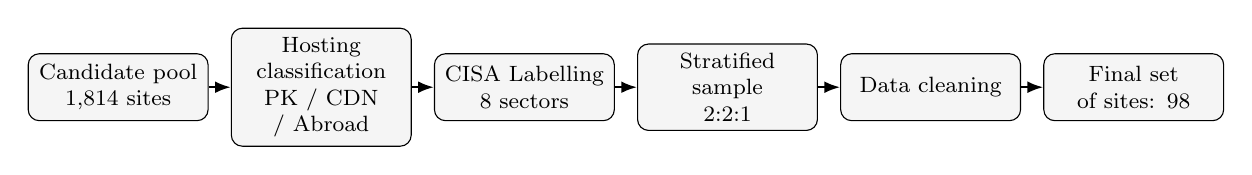
\begin{tikzpicture}[
      node distance=6pt and 8pt,
      stage/.style={draw, rounded corners, align=center, font=\footnotesize,
                    minimum height=0.85cm, text width=2.05cm, fill=black!4},
      arr/.style={-{Latex[length=2mm]}, thick}
    ]
    \node[stage] (s1) {Candidate pool\\1{,}814 sites};
    \node[stage, right=of s1] (s2) {Hosting\\classification\\PK / CDN / Abroad};
    \node[stage, right=of s2] (s3) {CISA Labelling\\8 sectors};
    \node[stage, right=of s3] (s4) {Stratified sample\\ 2:2:1};
    \node[stage, right=of s4] (s5) {Data cleaning\\};
    \node[stage, right=of s5] (s6) {Final set of sites: 98};
    \draw[arr] (s1) -- (s2);
    \draw[arr] (s2) -- (s3);
    \draw[arr] (s3) -- (s4);
    \draw[arr] (s4) -- (s5);
    \draw[arr] (s5) -- (s6);
  \end{tikzpicture}%
  }
  \caption {Site Selection Pipeline.}
  \label{fig:sample-pipeline}
\end{figure}



\paragraph{Location verification}
The above hosting classification is based on IP geolocation, which %is a widely used but imprecise method that 
maps IP addresses to approximate city-level locations.  we verify it against physics once measurements are available: no ping reply can arrive faster than the f-latency, the minimum round-trip time over fiber at the typical speed of light latency in fiber, so any measured RTT below that bound proves the claimed location wrong. Applied to the panel, this test invalidated the registered locations of 34 of the 40 CDN-class sites (anycast addresses whose registration city is, e.g., Toronto, yet which answer Pakistani probes in under 3\,ms) and corrected six unicast sites: three sites classed as Pakistani-hosted were in fact far from every probe (nearest ping 77--206\,ms,
consistent with their US and Singapore IP geolocation) and are reclassified as Abroad, and three sites
whose claimed city was physically impossible were relocated by latency multilateration, using each
probe's RTT as a distance bound. Each responding probe's RTT bounds the server to a circle of
radius $RTT/2$ at the fibre speed above, centred on that probe; the tightest (nearest-probe)
circle gives a hard existence bound, and an RTT-weighted centroid across all circles gives a point estimate whenever the nearest probe is within 20\,ms~\cite{gueye2006cbg}. The corrected hosting split is therefore 37 Pakistani, 40 CDN,
and 23 Abroad, and all per-class results below use the corrected classes. We treat this not as a
flaw in the sample but as a finding in its own right among the misclassified sites is a
provincial government service hosted in the United States---and as independent validation that
registration-based location data cannot be trusted at exactly the addresses this study cares
about.

The three sites reclassified from Pakistani to Abroad and the three relocated by multilateration
are found by different checks, not the same one run twice. The multilateration relocation above
starts from a proven impossibility: a reply faster than the physical floor cannot be explained
away, so it settles the question outright. A slow reply cannot be settled the same way, since it
is only implausible, never impossible, for a claimed-nearby site to answer slowly on a bad day. So
the second check is a threshold instead of a proof: a site labelled Pakistani whose nearest probe
still exceeds 20\,ms, further than any two points inside the country should plausibly be, has its
label corrected to Abroad. We checked for this direction specifically because a classifier built
on IP geolocation can misplace a distant server as easily as a nearby one, and three real
instances, out of 40 Pakistani-labelled sites, confirm that it does.\\
This check runs once the full seven-day panel has completed, not on a separate pilot deployment, and draws on every probe that returned a valid ping to the site in question, not a single vantage: each responding probe contributes its own distance-bounded circle to the multilateration estimate, and the 20ms threshold is evaluated against the nearest of them. We note one asymmetry in how rigorously the two directions of this correction are held: the Pakistani-to-Abroad relabelling above is decided by this RTT threshold alone, with no independent ASN or hop-level corroboration required in the classification pipeline itself. A stricter check, requiring a fresh ASN lookup and either a confirmed foreign hop or a foreign geo-IP city before relabelling, was run separately against all three affected sites (\texttt{phf.gop.pk}, \texttt{toptop.net}, \texttt{youth.cn}) and confirms the same result, but is not yet the standard the production pipeline enforces.

This is consistent with known limits of geolocation databases more broadly: Gharaibeh et al.~\cite{gharaibeh:imc:2011}  compare public and commercial geolocation services and found that accuracy degrades sharply below the country level, with metro- and city-level lookups substantially less reliable than coarse country-level classification — precisely the granularity our tromboning classification depends on, since a CDN anycast address registered to the correct country but the wrong city, or a unicast server whose registered city is merely implausible rather than wrong, would not be caught by a country-level check alone. This motivates verifying location against RTT physics directly (above) rather than relying on any geolocation database, however granular its claimed resolution.


\subsection{Vantage Points}
\label{sec:vantage}
% At the start of the experiment, 17 probes were live in Pakistan. We exclude one of these probes that was mislabeled with an incorrect ISP and was colocated with another probe. The remaining 
The locations of the 16 RIPE Atlas probes located in Pakistan that were live at the time of the experiment are shown in Figure~\ref{fig:probe-map}. The RIPE Atlas probe IDs, serving ISPs, and cities are shown in Table~\ref{tab:probes}.

% We measure from the RIPE Atlas probes connected within Pakistani networks at the time of the run, enumerated live from the platform API rather than from a fixed list, so that the vantage set reflects whichever probes are actually online, with each probe's ASN and location metadata verified against the platform API at analysis time rather than trusted from run-time labels. Seventeen probes were scheduled this way; sixteen returned data over the full week. Figure~\ref{fig:probe-map} shows where they are, and Table~\ref{tab:probes} lists every probe's ISP, city, and ASN. Several ISPs contribute more than one probe across multiple cities: Cybernet,
Nayatel, PTCL, and TES each have two or more vantage points, enabling within-ISP comparisons across locations. Data-quality caveats specific to individual probes (ICMP filtering, packet loss) are addressed in \S\ref{sec:cleaning}, once the measurement design
below establishes what each probe was asked to do.

\begin{figure}[t]
  \centering
  
\includegraphics[width=\columnwidth]{fig_probe_map.png}
  \caption{Vantage points by city. Bubble area is proportional to probe count.}
  \label{fig:probe-map}
\end{figure}

\subsection{Measurement Design}
\label{sec:measurement}
Against each of the 98 sites we run two complementary measurements from all the probes: a traceroute every hour and a ping every thirty minutes. %records the forward path once per hour; for each hop that returns an ICMP response, its IP address and cumulative round-trip time are recorded. An ICMP ping records end-to-end RTT and ICMP packet loss every thirty minutes; both fan out to all connected probes, and both run continuously for a seven-day window. 
We use Paris-style traceroute to TCP port~80 rather than ICMP for traceroute to reduce the effect of ICMP filtering and throttling. %is heavily filtered in Pakistani networks: 19 of the 37 Pakistani-class sites in our own sample never reply to ICMP at all (\S\ref{sec:prelim-ratio}), while the same hosts remain reachable over TCP/80. This affects only the destination: intermediate hops still reply (or not) via ICMP Time Exceeded regardless of the probe's transport, so switching to TCP/80 does not by itself recover hops that a router along the path declines to answer. We therefore use TCP/80 for the path measurement and additionally use Paris-style traceroute, which holds constant the header fields a load balancer hashes on, so that a change in the observed path is a genuine reroute and not an artifact of multipath forwarding.

Every ping measurement consists of three ICMP packets, so the ping measurement at time $t$ from probe $p$ to site $s$ results in a vector of RTT measurements: $\textbf{r}_{p, s, t} = [r_{p, s, t}^0, r_{p, s, t}^1, r_{p, s, t}^2]$, If any of the ICMP packets does not get a response, the corresponding RTT value is $NaN$. Similarly, each
traceroute measurement results in a vector $\textbf{h}_{p, s, t} = [\textbf{h}_{p, s, t}^0,
\textbf{h}_{p, s, t}^1, ..., \textbf{h}_{p, s, t}^{n_{p, s, t}}]$. Here $n_{p, s, t}$ is the
highest TTL value for which an ICMP packet was sent in that trace. Each $\textbf{h}_{p, s,
t}^i$ is itself a vector consisting of a hop IP address and the cumulative RTT value.

% The measurements are registered with RIPE Atlas as server-side \emph{periodic} instructions with a fixed start and stop, so that collection continues on the platform's own infrastructure independent of our host and a local collector can be restarted without loss of data. RIPE Atlas caps the number of simultaneously running measurements at one hundred per account; because one hundred sites each require both a traceroute and a ping, the run needs two hundred concurrent measurements, which we accommodate by splitting it across two accounts \emph{by measurement type}---one account carrying all one hundred traceroutes and the other all one hundred pings, against the identical site list and the same live-discovered probes. As the split is by type rather than by site, the merged dataset is identical to what a single unconstrained account would have collected.


\begin{table}[t]
\caption{RIPE Atlas probes used in the measurement panel.}
\label{tab:probes}
\begin{tabular}{llc}
\toprule
\textbf{ISP (ASN)} & \textbf{City} & \textbf{Probe ID}  \\
\midrule
Cybernet (9541)    & Haripur      & 1016036 \\
\    & Karachi      & 1016143    \\
\    & Karachi      & 1016154    \\
\hline Fasttel (150683)    & Islamabad    & 1014872  \\
\hline Nayatel (23674)    & Islamabad    & 60223     \\
\     & Islamabad    & 65892    \\
\hline Nova (136174)       & Lahore       & 1015679  \\
\hline Orbit (151983)      & Faisalabad   & 64535    \\
\hline PTCL (17557)       & Karachi      & 1016126   \\
\        & Mianwali     & 1016393  \\
\hline TES (135407)        & Rawalpindi   & 64078  \\
\         & Karachi      & 64722  \\
\hline Transworld (38193) & Lahore       & 62224  \\
\hline Zcom (152605)       & Lahore       & 7613     \\
\midrule
\textbf{Total} 9 ISPs & 7 cities & 14 probes \\
\bottomrule
\end{tabular}
\end{table}

\subsection{Data Cleaning}
\label{sec:cleaning}
The seven-day panel (11--18 July 2026) produced 218,480 traceroute rows and 436,828 ping records across the final 98-site sample. A total of 17 probes were scheduled, of which 16 returned data; after the two exclusions described below, 14 probes enter analysis with 200,292 traceroute rows and 305,116 ping rows. The active probes are given in Table~\ref{tab:probes}, covering both licensed international gateway operators and seven downstream ISPs.

One probe received no valid traceroute responses. We retain its ping RTT for latency analysis but exclude it from all hop-count and path-based analyses.

Another probe ran correctly for approximately 29 hours from the start of the experiment, then degraded to a bursty, intermittent connection for the remaining six days at roughly 5--10\% of normal rate. \hl{Its results are retained and included in the analysis, but any rate computed from it alone should be read against this thinner window.}

A third probe, distinct from the two above, had a 90\% packet loss throughout the run and is excluded from analysis entirely.

%For all ping records, we compute $r_{p, s, t} = \min\limits_{i}(r_{p, s, t}^i)$. 
Any ping record $\mathbf{r}_{p, s, t}$ with $\min\limits_{i}(r_{p, s, t}^i)$ of $NaN$ is dropped from the dataset. %We drop ping records with 100\% packet loss. 
We also drop traceroute records where $n_{p, s, t}$ is $255$. Furthermore, we drop the traceroute record $\mathbf{h}_{p, s, t}$ if any $\mathbf{h}_{p, s, t}^i$ has an RTT value exceeding 500\,ms. Finally, for tromboning analysis, we consider only records for probe-site pairs that have at least 50 traceroute records for statistical significance.

%The raw panel contains one row per measurement round per probe per target, with ping and traceroute rows stored together and distinguished by a \texttt{kind} column. For RTT analysis we use ping rows and drop any row where \texttt{rtt\_min} is NaN, corresponding to rounds with 100\% packet loss. For hop count analysis we exclude traceroute rows where \texttt{hop\_count} = 255, indicating the destination never replied. 
For each traceroute records $\mathbf{h}_{p, s, t}$ where $s$ is either a local site, or a CDN site with a cache available in Pakistan, tromboning is detected if there is a foreign geo-located IP address in the path.  In such cases, we determine the nearest Pakistani-owned hop preceding the first international-owned IP address and call it $\tau_{p, s, t}$. %field records which domestic ISP's hop preceded the RTT jump or foreign hop that triggered a trombone verdict. For a subset of trombone rows this handoff hop cannot be identified, 
If it can't be determined because the corresponding ICMP packets timed out, or the owning ASN can't be determined, the record is still retained because there is definite tromboning. %: the trombone, local, or inconclusive verdict is assigned from measured hop RTTs alone, independent of whether the handoff ISP could be identified. For the per-probe-site trombone fraction analysis we restrict to pairs with at least 50 rounds to ensure a statistically reliable estimate. Across the week, each probe--site pair accumulates roughly 336 ping rounds (one every 30 minutes), each of three packets, for about 1,000 individual RTT samples. As the latency measure feeding \S\ref{sec:ratio}, we take the single fastest packet observed for that probe--site pair over the full seven days---equivalently, the minimum of RIPE Atlas's per-round \texttt{rtt\_min} (itself the minimum of each round's three packets) taken across all rounds. A round in which every packet is lost yields no \texttt{rtt\_min} and is dropped before this minimum is taken, rather than contributing a value. Queuing and processing overhead only add delay on top of the true propagation time, so this minimum is the cleanest available approximation of the path's physical latency.~\cite{dibartolomeo2015}.

\subsection{The Latency Ratio}
\label{sec:ratio}
To compare RTTs between probe-site pairs involving varying geodesic distances, we adopt a normalization approach used in~\cite{bozkurt:dissecting:2018}. %We compute $r_{p, s, \bullet} = \min\limits_t{\mathbf{r}_{p, s, t}}$. This value is the cleanest available approximation of the path's physical latency.~\cite{dibartolomeo2015}. divide the RTT (measured by ping) by the "f-latency" (the minimum latency over a fiber optic cable given the geodesic distance between the probe and the site), giving a dimensionless \emph{latency ratio}: a value of $1$ means the path performs at its physical limit, and a value of $k$ means the connection takes $k$ times longer than the best possible. % Because the ratio is unitless it can be pooled across near and far sites and plotted as a distribution.%, and we retain the hosting class of every site so the distributions can be sliced by type. The theoretical minimum differs by class.
We scale the measured RTT values between all probe-site pairs down by the minimum possible RTT value.  
For PK or abroad sites, %\textbf{unicast sites} (the Pakistani and Abroad classes, one physical server each), 
the RTT values are scaled by f-latency (the minimum latency over a fiber optic cable given the geodesic distance between the probe and the site). With the probe and server coordinates, the great-circle distance $d$
follows from the Haversine formula~\cite{robusto:1957:cosine}. We assume the speed of light in optical fiber is $v_f = c/1.468 \approx 204{,}200$\,km/s, so the RTT values $r_{p, s, t}$ are replaced with $102 \frac{r_{p, s, t}}{d_{p, s}}$ where $d_{p, s}$ is the geodesic distance between probe $p$ and site $s$ measured in km.
% \begin{equation}
%   \mathit{RTT}_{0} \;=\; \frac{2d}{v_f} \;\approx\; \frac{d~[\mathrm{km}]}{102}~\mathrm{ms},
%   \qquad
%   \text{ratio} \;=\; \frac{\hat{\mathit{RTT}}}{\mathit{RTT}_0},
% \end{equation}
% where $\mathit{\hat{RTT}}$ is the minimum ping over the window (noise only ever adds
% delay, so the minimum best approximates the true path latency). 
To calculate $d_{p, s}$, probe coordinates are available from the RIPE Atlas API, while server coordinates are extracted using IP geolocation. %of the measured address (\S\ref{subsec:sites}). 
In cases where a probe is quite close a site ($d_{p, s} < 30 km$), the denominator of the latency ratio approaches $0$. In such cases, rather than calculate the latency ratio, the absolute value of the latency is retained in the dataset, but is not included when comparing latency ratios across probe-site pairs. The median value for such RTTs in our dataset is $5.6\,ms$. %are excluded from the ratio---the denominator approaches zero and the quotient degenerates---and are reported directly in milliseconds instead (their median in our data is 5.6\,ms, i.e.\ same-city delivery is healthy).

The above approach can not be directly applied to CDN sites because they don't have a single server location. Such $r_{p, s, t}$ values are scaled down by the minimum measured latency from any of the probes. Mathematically, the scaled RTT to CDN sites is $\frac{r_{p, s, t}}{\min\limits_{p, t}r_{p, s, t}}$. 

\hl{For CDN sites, no single server location exists, an anycast address is served from a different point of presence for each ISP, so there is no fixed coordinate from which to compute a physics-based floor the way unicast sites allow. We instead define the theoretical minimum empirically: the best RTT any Pakistani probe achieves to that site. This floor is attainable by construction, any ISP could in principle peer with the best-performing network, at the exchange this paper is about, and match its path, so the ratio measures exactly what an ISP loses by not peering, not distance. It requires no IP geolocation of the CDN edge, which we have already shown is unreliable for anycast addresses (\S\ref{subsec:sites}); the best-connected ISP scores $1$ and defines the frontier.}

\subsection{Tromboning Classification}
\label{sec:detector}
\hl{A naive classifier that flags any traceroute hop with foreign-registered IP ownership produces clear false positives: several routers physically inside Pakistan resolve to foreign-registered ASNs (median RTT $2.1\,ms$ from the nearest probe), most plausibly because operators acquired IPv4 address space on the open market rather than through the regional registrar, leaving the registration records unchanged. Two specific blocks account for nearly all of these cases and are excluded from country attribution by ASN: Shaw Communications (AS6327, Canadian-registered) and Cogent (AS174, US-registered), both confirmed physically present inside Pakistan by RTT and, for Shaw, a matching PTR record.}

\hl{A traceroute round is classified as \emph{tromboned} if and only if at least one responding hop satisfies all of the following: (1) it resolves to a real, non-\texttt{PK} country; (2) it is not a private address; (3) its ASN is not on the artifact list above; (4) it actually responded, a timed-out hop is skipped, not treated as foreign; and (5) its own RTT falls between $40\,ms$ and $500\,ms$. The lower bound is not a distance calculation to a named exchange; it is calibrated from the observed ceiling of purely domestic Pakistani RTT, which does not exceed roughly $40\,ms$ anywhere in our data, while confirmed foreign hops (Singapore, the United States) never answer below $60\,ms$. The upper bound discards hop RTTs above $500\,ms$ as queuing or ICMP-error-generation artefacts, common on the ICMP-filtered probes. If no hop satisfies all five conditions, the round is classified local, regardless of maximum end-to-end RTT or the size of any jump between hops: RTT alone, without a resolvable foreign hop, is not treated as evidence a trace left the country.}

\hl{This is stricter than an earlier version of the detector that also flagged a round as tromboned on RTT signals alone (a $\geq\!60\,ms$ jump between hops, or any hop $\geq\!70\,ms$, with no foreign hop required). We removed that path because domestic congestion can produce the same RTT signature as a genuine foreign detour, so it cannot distinguish the two; every number in \S\ref{sec:results} below uses the confirmed-hop-only rule.}
 

%A naive classifier for tromboning examines the traceroute to a Pakistani hosted site for any IP address with a foreign-entity ownership using the Whois database, and classifies it as tromboning. However, our collected data showed clear false positives. Several IP addresses appear to be in use on routers inside Pakistan, as evidenced by small RTTs (a median RTT of $2.1\,ms$ from one of our probes, for instance), that are registered to foreign entities. Conversations with operators indicate that these may be due to operators acquiring IPv4 addresses from the open market, rather than the Internet registrars, and the registrar entries not having been updated. An examination of the traceroutes in our dataset showed that the smallest recorded RTT for any link between a router in Pakistan and the other abroad is $45\,ms$.
%
%We manually inspected the naive classifier's results to get more conservative results. If the hop labelled by IP geolocation as foreign, is sandwiched between two Pakistani routers, and the incremental RTT is lower than $45\,ms$, we label that traceroute as not tromboning. Our classifier may have some false negatives, but it is better to err on the side of caution.
\section{Results}
\label{sec:results}
The week-long run completed on 18~July~2026. %; the traceroute and ping halves are merged on probe, site, and round, and all results below are computed on the full, cleaned week (\S\ref{sec:cleaning}): 204,384 traceroutes and 313,276 pings from 14 probes. 
The week was event-free---no submarine cable fault or
publicly reported routing incident overlaps the window, and the daily tromboning rate varies only
between 14.5\% and 15.9\%, so the numbers below describe the steady state of Pakistani routing
rather than an anomaly. These measurements double as the normal-day baseline for future event studies. We
first present two normalised cross-sections (the latency ratio and the CDN grid), then the three
analyses the panel was designed for, one per research question.

Throughout, we report four indicators per probe--site pair, matching the metric set of prior IXP
measurement work~\cite{dibartolomeo2015}: minimum round-trip time (the primary latency measure,
\S\ref{sec:cleaning}); jitter, the standard deviation of round-trip time over all rounds for that
pair ($\sigma_{p,s,\bullet}$); ICMP ping packet loss, the fraction of ping packets that go
unanswered; and hop count, from the traceroute half.

\hl{Packet loss averages 23.9\% across all valid ping rounds, driven almost entirely by destination policy rather than path quality: Pakistani-class sites lose 48.3\% of packets, consistent with the 19 of 37 that block ICMP outright, against 16.6\% for Abroad and 3.0\% for CDN sites; loss is otherwise flat across ISPs (23.2--24.9\%). Jitter, the standard deviation of minimum RTT across rounds for a pair, has a median of 7.45\,ms (1,092 pairs with at least two valid rounds); every ISP falls between 1.5 and 14.2\,ms except PTCL, whose 112.5\,ms median is attributable entirely to its Mianwali vantage (139.4\,ms) and not its Karachi vantage (6.15\,ms). Hop count has a median of 10 across 143,861 valid traceroutes, 14 for Abroad sites, 10 for CDN and Pakistani sites; Nayatel is an outlier at a median of 2 hops, consistent with its direct peering noted elsewhere. Hairpinned Pakistani-hosted traces run a median 11 hops against 10 for local traces} (Figure~\ref{fig:rtt-indicators}).

\begin{figure}[t]\centering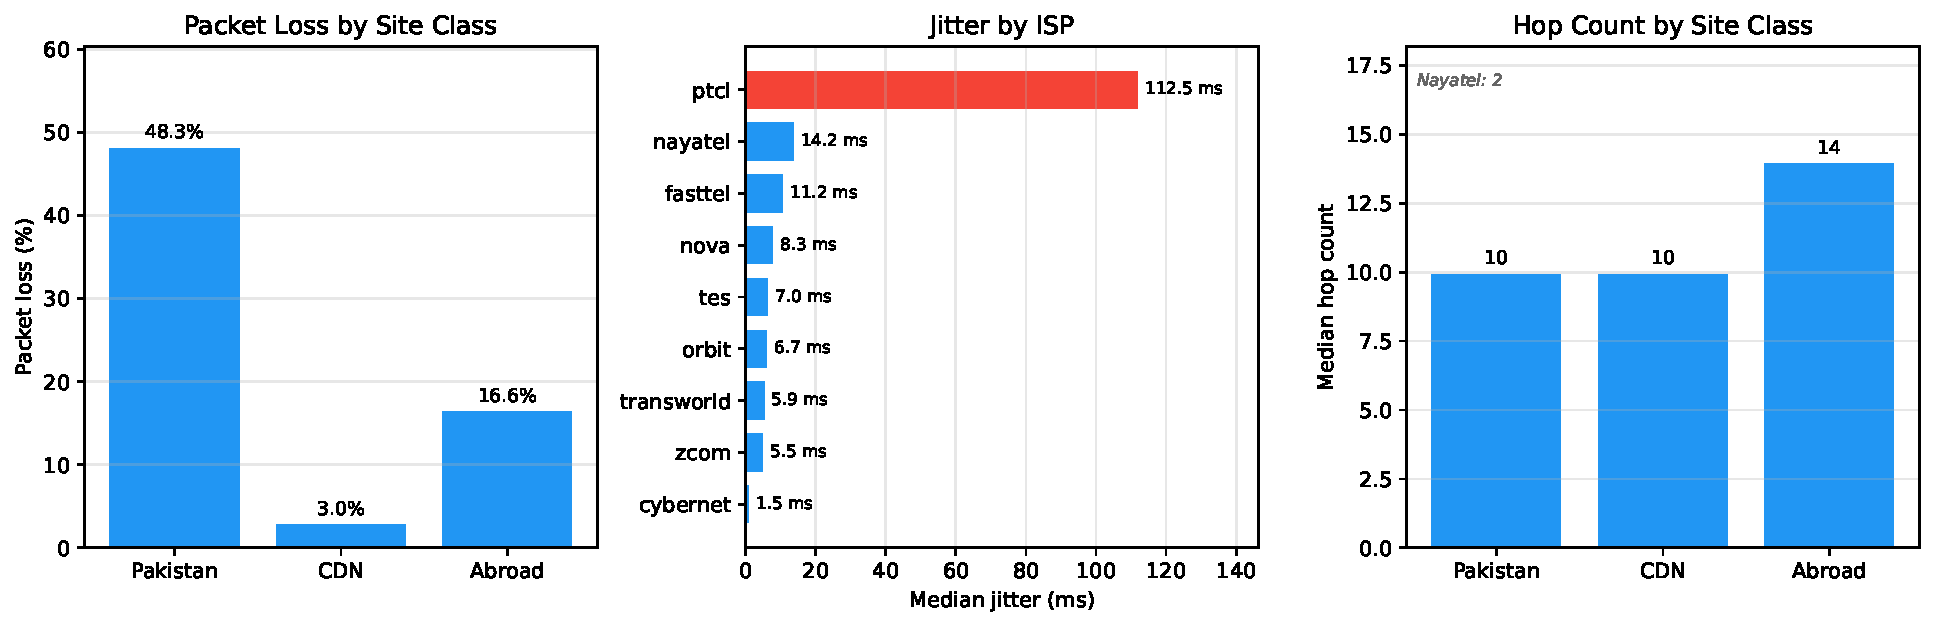
\includegraphics[width=\columnwidth]{fig_rtt_indicators.pdf}
  \caption{Packet loss by site class, jitter by ISP (PTCL's outlier is its Mianwali vantage, not Karachi), and hop count by site class.}\label{fig:rtt-indicators}\end{figure}

\subsection{Latency Ratio by Site Type}
\label{sec:prelim-ratio}
Figure~\ref{fig:ratio-cdf} shows the distribution of the latency ratio (\S\ref{sec:ratio}) for the 486 probe--site connections to unicast sites with a ping response and the 546 connections to CDN sites, as cumulative distribution functions. Furthermore, latency ratios for \emph{Pakistani} sites have a median value of 2.98$\times$, but carry a heavy tail: 26.6\% of pairs exceed 10$\times$, reaching 75.17$\times$. The tail is not dominated by any one vantage's noise: /hl{Cybernet's Haripur probe produces the single most extreme values} (up to 75.17$\times$), all short (30--40\,km), same-city pairs where its own last-mile floor collides with a near-zero theoretical minimum, the same access-floor-inflation effect already discussed above; Orbit has the highest \emph{share} of its own pairs in the tail (61\% exceed 10$\times$, though less extreme individually, 27--31$\times$); PTCL, both vantages combined, sits at 26.7\%, indistinguishable from the sample-wide 26.6\%, not a standout despite Mianwali's known data-quality caveats elsewhere. [...]

We perform a regression analysis of the measured RTTs against geodesic distance, separately for Pakistani and Abroad sites (Figure~\ref{fig:distance-regression}). For Abroad sites, distance explains most of the variation in RTT ($R^2=0.48$, $p<10^{-40}$), consistent with latency that tracks how far the packet actually travels. For Pakistani sites, distance explains almost none of it ($R^2=0.022$, $p=0.01$). A domestic site 1,000\,km away is not
reliably slower than one 100\,km away. Distance is not the variable driving intra-country latency. This may be due to path tromboning as discussed in \S\ref{sec:rq1}. The delay may be due to routing choices, not a function of geography. 

\begin{figure}[t]
  \centering
  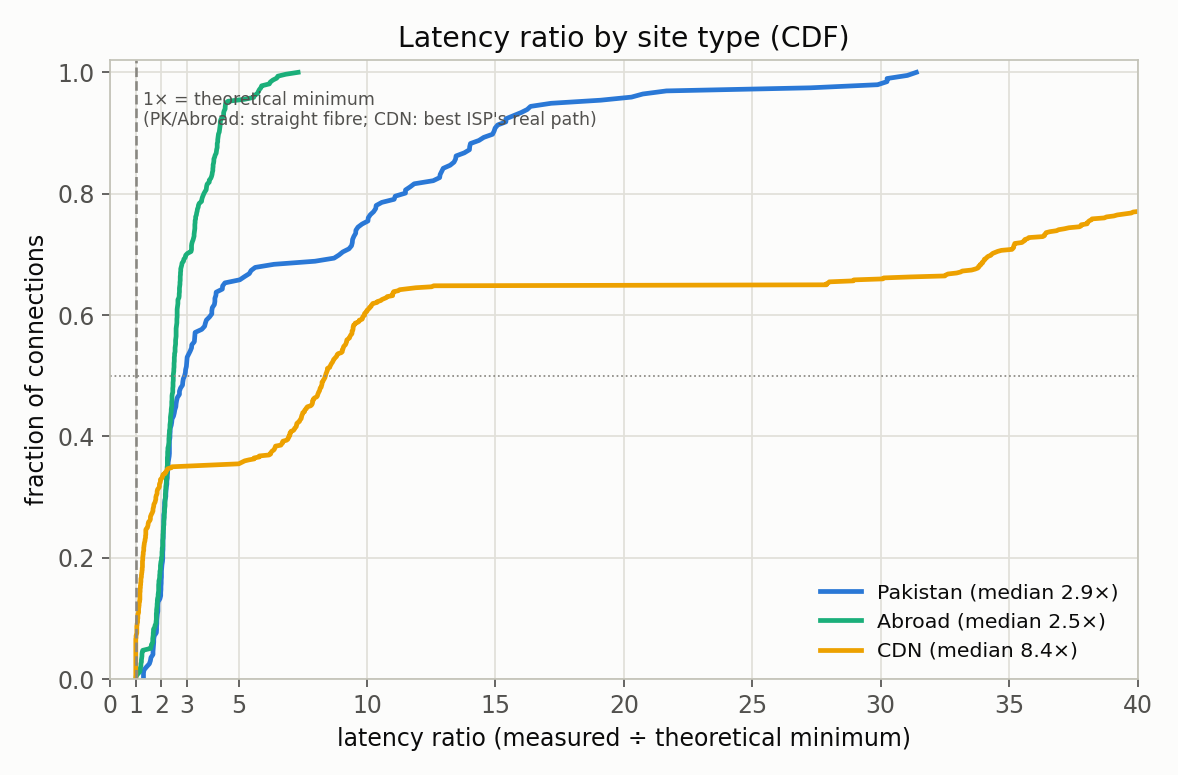
\includegraphics[width=\columnwidth]{ratio_cdf_all3.png}
  \caption{%Latency ratio by site type (full week). For Pakistani and Abroad sites the theoretical minimum is straight fibre over the verified great-circle distance; for CDN sites it is the best RTT any Pakistani probe achieves (\S\ref{sec:ratio}). Foreign sites are uniform; Pakistani sites carry a long tail; CDN access is bimodal.
  Latency ratio from all probes by site location. Sites hosted abroad show the smallest variation. Pakistani sites exhibit a long tail and CDN hosted sites show bi-modal behavior.}
  \label{fig:ratio-cdf}
\end{figure}

\begin{figure}[t]
  \centering
  \begin{subfigure}[b]{0.48\columnwidth}
    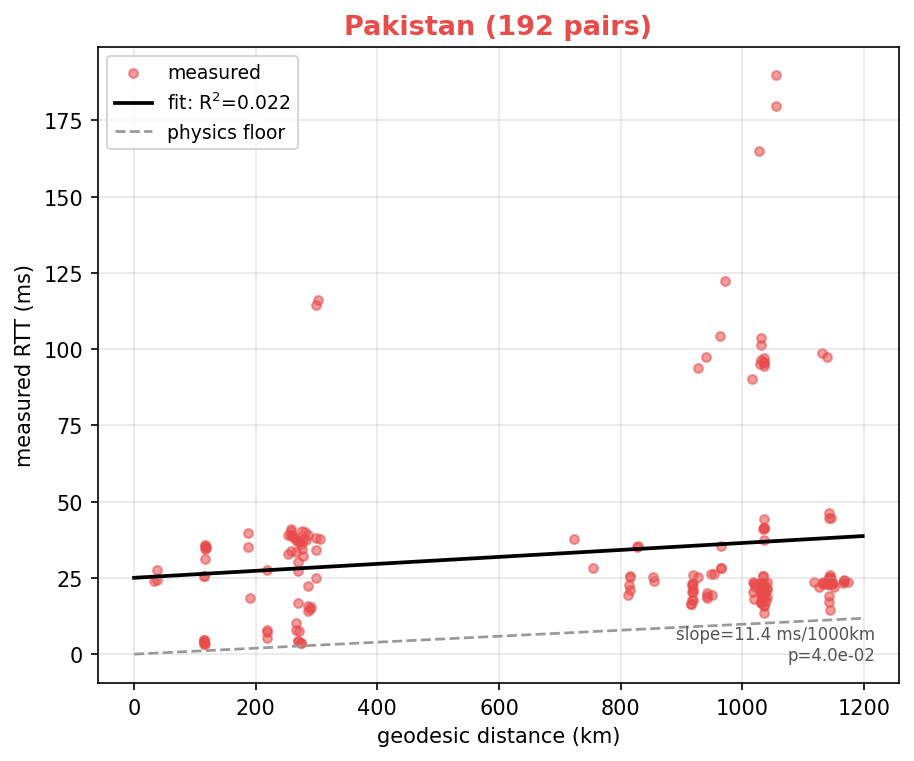
\includegraphics[width=\linewidth]{fig_distance_regression_pk.png}
    \caption{Pakistan (192 pairs)}
    \label{fig:distance-regression-pk}
  \end{subfigure}
  \hlill
  \begin{subfigure}[b]{0.48\columnwidth}
    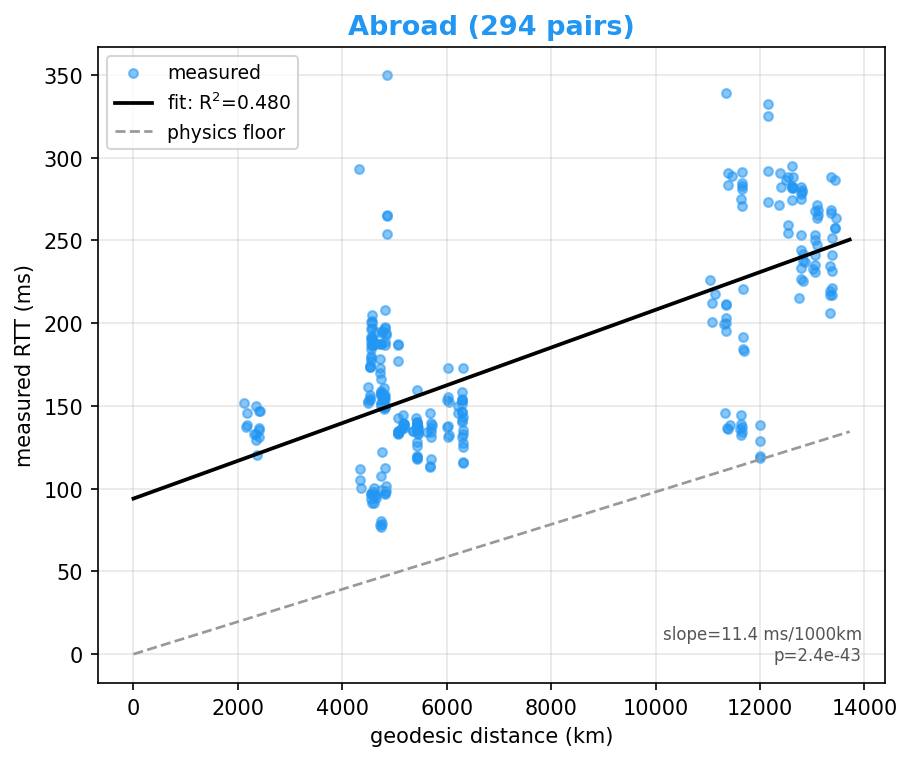
\includegraphics[width=\linewidth]{fig_distance_regression_abroad.png}
    \caption{Abroad (294 pairs)}
    \label{fig:distance-regression-abroad}
  \end{subfigure}
  \caption{Measured RTT against geodesic distance, fitted separately per class (same 486
  intercity unicast pairs as Figure~\ref{fig:ratio-cdf}). The dashed line is the physics floor.
  Abroad RTT tracks distance closely; Pakistani RTT does not, ruling out a pure base-effect
  explanation for the ratio tail above.}
  \label{fig:distance-regression}
\end{figure}

\subsection{The CDN Cross-Section---the Local Path Exists}
\label{sec:prelim-cdn}
RQ3 asks whether a local path exists for traffic that nonetheless leaves the country. %and answers it longitudinally, through verdicts that flip over the week. The CDN measurements already answer the same question \emph{cross-sectionally}. 
We define three RTT cut-offs for CDN cache access: local ($<$15\,ms), regional (15--50\,ms), or far ($>$50\,ms), the same tiers used throughout this paper's CDN treatment. Figure~\ref{fig:cdn_by_isp} shows the fraction of CDN-hosted site accesses, grouped by ISP, that reach a local, regional, or far cache.
%We define three latency cut-offs for CDN cache access: local ($<$15\,ms), regional (15--50\,ms), or far ($>$50\,ms). Figure~\ref{fig:cdn_by_isp} shows the fraction of CDN-hosted site accesses, grouped by ISP that access a local, regional or far cache.
%, the latency to the CDN cache that serves that ISP is: local ($<$15\,ms), regional (15--50\,ms), or far ($>$50\,ms). %thresholds we calibrated in earlier cache-presence work.  The rows order themselves into a peering ranking:
All ISPs appear to find a regional cache around 40\% of the times. Only three ISPs in our dataset find local caches. The best-case ISP reaches 85\% of CDN content locally or regionally, with a median latency of 2.7\,ms. In contrast, the ISPs that don't find a local cache, have median RTTs of 91--130\,ms. Expressed with the CDN ratio of \S\ref{sec:ratio}, the median
cost of non-peering ranges from $2\times$ (second-best network) to $12.7\times$ (the largest
operator), and the worst quarter of ISP--site pairs exceed $40\times$. 

This exposes how low the level of local peering among Pakistani ISPs is. The longitudinal version follows in
\S\ref{sec:rq3}.

Some of the sites in red are those that use DDoS prevention mechanisms abroad. CDN operators don't have local deployment available for that. Conversations with staff at a major Pakistani ISP revealed a lack of DDoS prevention solutions availability in the market until very recently. That operator has now acquired the capability, but competing against established international players is an uphill task. Even if we discount for the necessity of DDoS prevention being impossible locally, this still makes a good case for significant experience improvements that are possible through better utilization of the IXPs. 

\hl{The obvious follow-up is how much this would actually save each ISP. Taking Nayatel's mean CDN RTT (20.3\,ms) as the "ideal peering" benchmark, the fleet-wide mean would fall from 70.2\,ms to 20.3\,ms, a 71\% reduction, if every ISP matched it. The saving is not uniform: Cybernet, already the second-best-peered network, would gain the least (32.4\,ms, 61.5\% reduction), while PTCL, the largest operator, would gain the most (116.0\,ms, 85.1\% reduction). Table~\ref{tab:cdn-savings} gives the full breakdown. The ordering matters for where incentives should focus: the ISPs with the most to gain from peering properly are the ones currently peering worst, not the smaller networks already closest to the frontier.}

\begin{table}[t]
\caption{Mean CDN RTT per ISP against the best-peered network (Nayatel, 20.3\,ms), and the reduction each ISP would see under equivalent peering.}
\label{tab:cdn-savings}
\begin{tabular}{lrrr}
\toprule
\textbf{ISP} & \textbf{Mean RTT (ms)} & \textbf{Decrease (ms)} & \textbf{Reduction} \\
\midrule
Nayatel     &  20.3 &   0.0 & --    \\
Cybernet    &  52.7 &  32.4 & 61.5\% \\
TES         &  63.1 &  42.8 & 67.8\% \\
Zcom        &  65.6 &  45.3 & 69.1\% \\
Orbit       &  68.0 &  47.7 & 70.1\% \\
Nova        &  69.2 &  48.9 & 70.7\% \\
Transworld  &  71.7 &  51.4 & 71.7\% \\
Fasttel     & 111.1 &  90.8 & 81.7\% \\
PTCL        & 136.3 & 116.0 & 85.1\% \\
\bottomrule
\end{tabular}
\end{table}

% \begin{figure}[t]
%   \centering
%   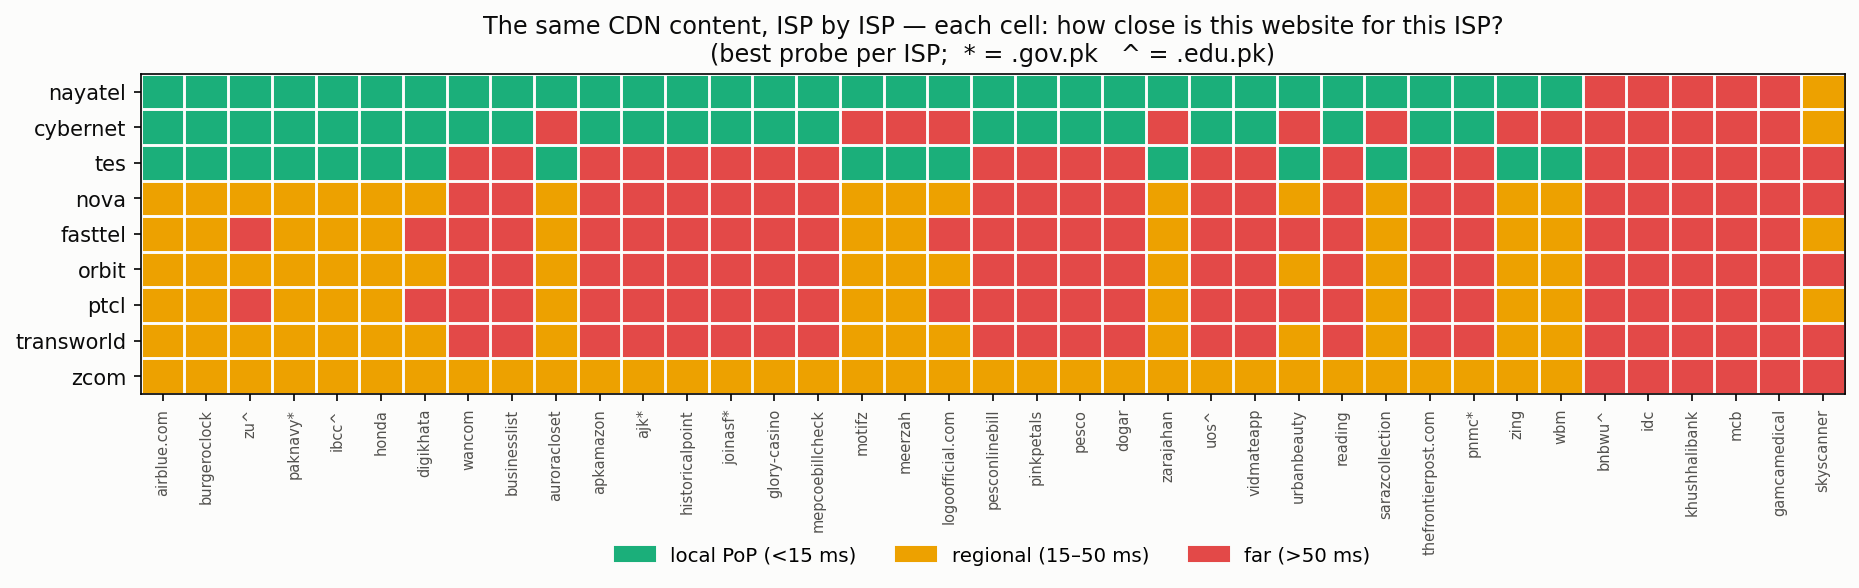
\includegraphics[width=\columnwidth]{cdn_heatmap.png}
%   \caption{CDN access grid (full week, best probe per ISP). Green: served from a local PoP
%   ($<$15\,ms); amber: regional (15--50\,ms); red: far ($>$50\,ms). Rows form a peering ranking;
%   solid-red columns are sites fronted offshore for every ISP.}
%   \label{fig:cdn-heatmap}
% \end{figure}

\begin{figure}[t]
  \centering
  
\includegraphics[width=\columnwidth]{cdn_by_isp.png}
  \caption{CDN access by ISP}
  \label{fig:cdn_by_isp}
\end{figure}

% \begin{table}[t]
% \caption{CDN sites by best-case reachability: the closest PoP distance any of the 9 ISPs
% achieves for that site.}
% \label{tab:cdn-bestcase}
% \begin{tabular}{lrrl}
% \toprule
% \textbf{Best case} & \textbf{Sites} & \textbf{\%} & \textbf{Examples} \\
% \midrule
% Always far ($>$50\,ms for every ISP)      & 5  & 12.8\% & mcb.com.pk, khushhalibank.com.pk \\
% Sometimes regional (15--50\,ms best case) & 1  & 2.6\%  & skyscanner.pk \\
% Sometimes near ($<$15\,ms best case)      & 33 & 84.6\% & airblue.com, ajk.gov.pk \\
% \bottomrule
% \end{tabular}
% \end{table}

\begin{table}[t]
\caption{CDN sites by best-case reachability: the closest PoP distance any of the 9 ISPs
achieves for that site. Always-far examples: mcb.com.pk, khushhalibank.com.pk; the sole
regional-best site is skyscanner.pk.}
\label{tab:cdn-bestcase}
\begin{tabular}{lrr}
\toprule
\textbf{Best case} & \textbf{Sites} & \textbf{\%} \\
\midrule
Always far ($>$50\,ms, every ISP)     & 5  & 12.8\% \\
Sometimes regional (15--50\,ms best)  & 1  & 2.6\%  \\
Sometimes near ($<$15\,ms best)       & 33 & 84.6\% \\
\bottomrule
\end{tabular}
\end{table}


\subsection{Extent and Attribution of Tromboning (RQ1)}
\label{sec:rq1}
\hl{Over the course of the week, 5.52\% of the 75,600 analyzed traces destined for Pakistani-hosted sites left the country before returning. This rate is notably lower than the 13\% reported by Edmundson et al.\ for Brazil, the 50\% for Kenya, and the 66.8\% measured by Gupta et al.\ for intra-African paths~\cite{edmundson2016characterizing, gupta2014}.}

This hairpinning rate is driven far more by the vantage point than by the actual destination, as demonstrated by the breakdown of confirmed hairpins across operators (Figure~\ref{fig:panel-source}):
\begin{itemize}
    \item Nayatel and Transworld both show zero confirmed hairpins throughout the week.
    \item Cybernet sits at 2.6\%.
    \item Fasttel, Nova, Orbit, and TES cluster together at 8.1\%.
    \item Zcom comes in at 8.2\%.
    \item PTCL, the largest operator, reaches 11.3\%.
\end{itemize}

\hl{The previously observed threshold rule turns out to be an artifact of the measurement technique rather than a genuine routing difference. When evaluated under the confirmed-hop standard, PTCL's Karachi and Mianwali vantages sit at 11.0\% and 12.5\%, compared to 46\% and 27\% previously. Similarly, Cybernet's Haripur and Karachi vantages now measure 5.4\% and 0.0\%, down from their prior 34\% and 11\%. While a modest, city-dependent gap still exists for both ISPs, the dramatic swings produced by the RTT-alone rule disappear once a confirmed foreign hop is required.}

\hl{Out of 4,170 confirmed hairpins, every single trace resolves to a hand-off distributed among five primary providers: Transworld leads with 1,825, followed by PTCL (949), TES (503), Cybernet (336), and Orbit (166).}

\hl{This traffic exits through a heavily concentrated geography. Singapore accounts for the vast majority with 3,740 traces, largely driven by an Equinix egress, while the United States (253) and Hong Kong (167) trail as a distant second and third. Notably, the sharp drop in US-attributed traces compared to earlier counts stems from the correction of a Cogent router based in Pakistan that was previously misread as a US exit.}

When examined by sector, the vulnerability landscape shifts dramatically:
\begin{itemize}
    \item Financial Services is by far the worst-routed sector in the country, with an alarming 58.3\% of traces to Pakistani-hosted banking sites hairpinning.
    \item Government Services follows at 14.6\%.
    \item Commercial Facilities registers at 1.4\%.
    \item Every other sector shows zero confirmed tromboning under this standard.
\end{itemize}

\hl{Most crucially, a hop-by-hop scan of all 222,944 traces against the peering-LAN prefixes of PKIX Lahore and PIE Karachi revealed zero traces crossing either exchange fabric during the entire week. Instead, 11,756 traces destined for domestic locations detoured entirely through Singapore or the United States, completely bypassing the local paths the exchange infrastructure was built to serve.}

\hl{\textbf{5.52\% is a lower bound, not a point estimate.} The detector can only confirm a trace tromboned via a hop that actually responds; it can never falsely confirm one from a gap. 65.2\% of Pakistani-class traces (49,285 of 75,600) contain at least one hop that never responds before the last hop we can classify, so for most traces some portion of the path is simply invisible to us. We cannot bound how much this undercounts the true rate from this fact alone. As a targeted, corroborated check, not a blanket RTT-based rule, we reclassified a trace as tromboned if it has such a gap \emph{and} its destination-hop RTT falls within the 5th--95th percentile of destination RTT already confirmed for that exact site by other, fully-visible rounds. This only ever applies to the 8 sites (of 37) with at least one confirmed-trombone round to corroborate against, it cannot and does not move the other 29. Under this check the rate rises to \textbf{8.3\%} (6,279/75,600); we report it as a named robustness bound, not a replacement for the confirmed-hop headline, since it reintroduces RTT as evidence, corroborated by same-site observations rather than a bare threshold, a weaker standard than the rest of this paper holds to.}
\begin{figure}[t]\centering
\includegraphics[width=\columnwidth]{fig_trombone_by_isp.pdf}
  \caption{Tromboning rate per vantage (ISP and city) over the full week, PK-hosted sites only.}\label{fig:panel-source}\end{figure}

\subsection{The Latency Cost and Its Stability (RQ2)}
\label{sec:rq2}
% Local traces to Pakistani-hosted sites have a median minimum RTT of 24.5\,ms; hairpinned traces to
% the same class of site have a median of 104.3\,ms (Figure~\ref{fig:panel-cdf}). This gap is
% descriptive, not causal: it compares two different populations of sites, some structurally near
% and some structurally far, rather than measuring what happens when the \emph{same} site's traffic
% takes one path instead of the other.

% To isolate the causal cost, we use the 121 probe--site pairs that flip between local and
% hairpinned verdicts within the week and have a measured RTT in both states. For these pairs,
% taking the hairpin instead of the local path adds a median of just $+0.5$\,ms. The mean is far
% higher, $+15.3$\,ms, because a few pairs pay a large penalty and most pay almost none: for the
% majority of flapping traffic, the detour itself is close to latency-free.

% [Correction 11a] Local-vs-hairpinned median RTTs updated (24.5/104.3 -> 25.1/118.0ms) under the final 5-rule detector.
\hl{Local traces to Pakistani-hosted sites have a median minimum RTT of 25.1\,ms; hairpinned traces to
the same class of site have a median of 118.0\,ms (Figure~\ref{fig:panel-cdf}). This gap is
descriptive, not causal: it compares two different populations of sites, some structurally near
and some structurally far, rather than measuring what happens when the \emph{same} site's traffic
takes one path instead of the other.}

% [Correction 11b] Causal flip-pair estimate dropped: sample collapsed 121->7 pairs under the stricter detector, too few to trust, so we report the descriptive comparison instead of forcing a causal number.
\hl{Isolating the causal cost is no longer statistically viable under the confirmed-hop standard:
only 7 probe--site pairs flip between local and hairpinned verdicts within the week and have a
measured RTT in both states, too few for a reliable estimate (mean $-2.3$\,ms, i.e.\ noise, not a
finding). We report the round-level descriptive comparison above as this section's evidence rather
than force a per-pair causal estimate from an underpowered sample.}

The latency case against tromboning therefore rests on a smaller, structural minority rather than
on this flapping majority. Pairs that are hairpinned on nearly every round sit at roughly
100\,ms against a roughly 25\,ms local norm, and the CDN gap (\S\ref{sec:prelim-cdn}) is larger
still. What the near-free majority of flips costs is not milliseconds but \emph{exposure}: every
hairpinned packet depends on the same submarine cable and licensed international gateway, exactly
the infrastructure a cable fault degrades, and the transit whose cost is paid in foreign exchange
(\S\ref{sec:discussion}).

% [Correction 11c] Trombone-rate-over-time figures updated (13.6-16.5% hourly / 14.5-15.9% daily -> tight 4.5-4.8% / 4.6-5.1% bands) under the final detector.
\hl{The tromboning rate is stable over time, more so under this standard than the earlier one,
which rules out congestion as the cause. Hourly, it ranges from 4.5\% to 4.8\% across the day.
Daily, it stays within 4.6--5.1\% across all seven days, with no weekday--weekend difference.}


% The tromboning rate is stable over time, which rules out congestion as the cause. Hourly, it
% ranges from 13.6\% at 06:00~PKT to 16.5\% at 23:00~PKT, under 3 percentage points of absolute
% variation. Daily, it stays within 14.5--15.9\% across all seven days, with no weekday--weekend
% difference. 

A profile this flat means the penalty comes from where content is hosted and how it
is routed, not from how busy the network is at a given moment, so the remedy is local hosting
and peering, not additional capacity.

As a secondary check, on a three-day snapshot we recomputed the ratio after subtracting each
probe's own last-mile floor (its fastest observed RTT to any Pakistani site), isolating the path
itself from the access link. Under this path-only view, the Pakistani median ratio drops from
2.9$\times$ to 1.9$\times$, below the foreign 2.4$\times$: the typical domestic \emph{route}, once
the local access overhead is removed, is efficient. The inefficiency measured above lives
specifically in the access link and in the tail, not in the ordinary domestic path.
\begin{figure}[t]\centering
\includegraphics[width=\columnwidth]{fig_local_vs_hairpin_cdf.pdf}
  \caption{CDF of min-of-$N$ RTT to Pakistani-hosted sites, local vs hairpinned traces.}\label{fig:panel-cdf}\end{figure}

\subsection{Existence of a Local Path (RQ3)}
\label{sec:rq3}
% Of the 444 probe--site pairs on Pakistani-hosted sites with at least 50 rounds, 211 (48\%) are
% persistently local, 40 (9\%) are persistently hairpinned, and 193 (43\%) \emph{flap}: the same
% probe reaching the same site is served domestically on some rounds and via a foreign detour on
% others, within the same week. In the terms RQ3 poses: \textbf{83\% of the pairs that ever trombone
% are also served by a domestic path during the week}---for the overwhelming majority of hairpinning
% traffic, the international detour is a routing choice, not a necessity. The site-level view is
% starker still: every one of the 37 Pakistani-hosted sites was hairpinned on at least one round
% from at least one vantage, 35 of 37 flap, and only two sites are hairpinned on more than 90\% of
% rounds---the sites for which no usable local path may exist. The choice extends to the gate
% itself: 23 pairs were handed to \emph{both} PTCL and Transworld at different times in the week for
% the same destination. Hop-level analysis of consecutive rounds localises the mechanics: 78\% of
% path divergence occurs at hops 3--5---the domestic aggregation and pre-gateway layer, the exact
% segment an exchange would replace---detours toggle on and off symmetrically rather than migrating
% (96\% of changing pairs return to a previously observed route), and 49\% of all pairs genuinely
% re-route at the AS level at least once during the week. The tromboning rate is therefore best
% stated as a stable weekly range, 14.5--15.9\%, produced not by a fixed set of broken routes but by
% a continuously flapping choice between a local path and a foreign one.

% [Correction 12] RQ3 rewritten: hairpinning is now rare & concentrated (415 local/16 hairpinned/13 flap, was 211/40/193), not near-universal. Trailing "14.5-15.9% weekly range" sentence dropped (contradicted the new ~5% rate; not in the md's own draft, added here for consistency).
\hl{Of the 444 probe--site pairs on Pakistani-hosted sites with at least 50 rounds, 415 (93.5\%) are
persistently local, 16 (3.6\%) are persistently hairpinned, and 13 (2.9\%) \emph{flap}: the same
probe reaching the same site is served domestically on some rounds and via a confirmed foreign
detour on others, within the same week. Of the 29 pairs that ever trombone, hairpinned or
flapping, \textbf{44.8\% are also confirmed local at other times in the same week}, evidence that a
domestic path exists for close to half of hairpinning traffic, though a smaller share than an
earlier, RTT-threshold-based estimate suggested. The site-level view is the more striking result
under this standard: only 8 of the 37 Pakistani-hosted sites were ever confirmed hairpinned on any
round from any vantage, the remaining 29 (78\%) stayed local on every confirmed round all week. The
same 8 sites account for all of the flapping behaviour; none is hairpinned on more than 90\% of
rounds. Hairpinning under this standard is therefore not a general property of Pakistani hosting,
it is concentrated in a small, identifiable minority of sites, consistent with RQ1's sector
attribution, Financial Services and Government Services account for nearly all of it.}

\hl{Hop-level analysis of the 70 verdict-flip transitions we can compare directly finds 46.7\% of
the 45 resolvable divergences occur at hops 3--5, the domestic aggregation and pre-gateway layer.
Requiring the stricter test of a genuine AS-path reroute, not explainable by a hop simply timing
out, 14.9\% of the 444 pairs (66) show at least one such reroute across the week, and 5.7\% of
individual verdict-flip transitions (4 of 70) are path-confirmed rather than hop-visibility
artefacts.}

\subsection{Similarity of User Experience Within a City (RQ4)}
\label{sec:rq4}
\hl{Research Question 4 examines whether users subscribed to different ISPs within the same city experience similar latency when accessing locally available content. The data clearly shows that they do not, and because the city remains constant, physical distance can be completely ruled out as the cause for this discrepancy.}

\hl{For example, in Karachi, four vantage points access the same CDN-hosted sites with drastically different median latencies. Cybernet achieves 4.4\,ms (with 61.5\% served locally), TES records 78.0\,ms (41.0\% local), and PTCL trails at 129.8\,ms (0.0\% local). This creates a 29.8$\times$ spread between the fastest and slowest ISPs operating in the exact same city. Lahore demonstrates this identical pattern. Nayatel achieves a median latency of just 2.8\,ms (with 84.6\% of content served locally). In contrast, Nova, Transworld, and Zcom all cluster between 91 and 95\,ms with absolutely zero local hits, resulting in a staggering 34$\times$ spread (Figure~\ref{fig:rq4-same-city}).}

\hl{This observation aligns with and even magnifies the country-wide CDN gap detailed in \S\ref{sec:prelim-cdn}, which ranged from $2\times$ to $12.7\times$ across all nine ISPs. When the scope is restricted to a single city where the physical distance to any given CDN point of presence is effectively identical for every vantage point, the performance gap actually widens.}

\hl{Therefore, the driving variable behind this disparity is peering rather than geography. The faster ISPs in each city, specifically Cybernet and Nayatel, have successfully connected to a local cache. Meanwhile, the slower ISPs have not, despite being physically no further away.}

\hl{This is precisely the type of structural asymmetry an internet exchange is built to eliminate. Resolving this issue does not require moving any users, laying new cable, or changing content hosting locations. It simply requires the slower ISPs in each city to adopt the same peering practices as the fastest ones. Once implemented, every user in that city would inherit the same low latency currently enjoyed exclusively by customers of the best-connected networks.}

\begin{figure}[t]\centering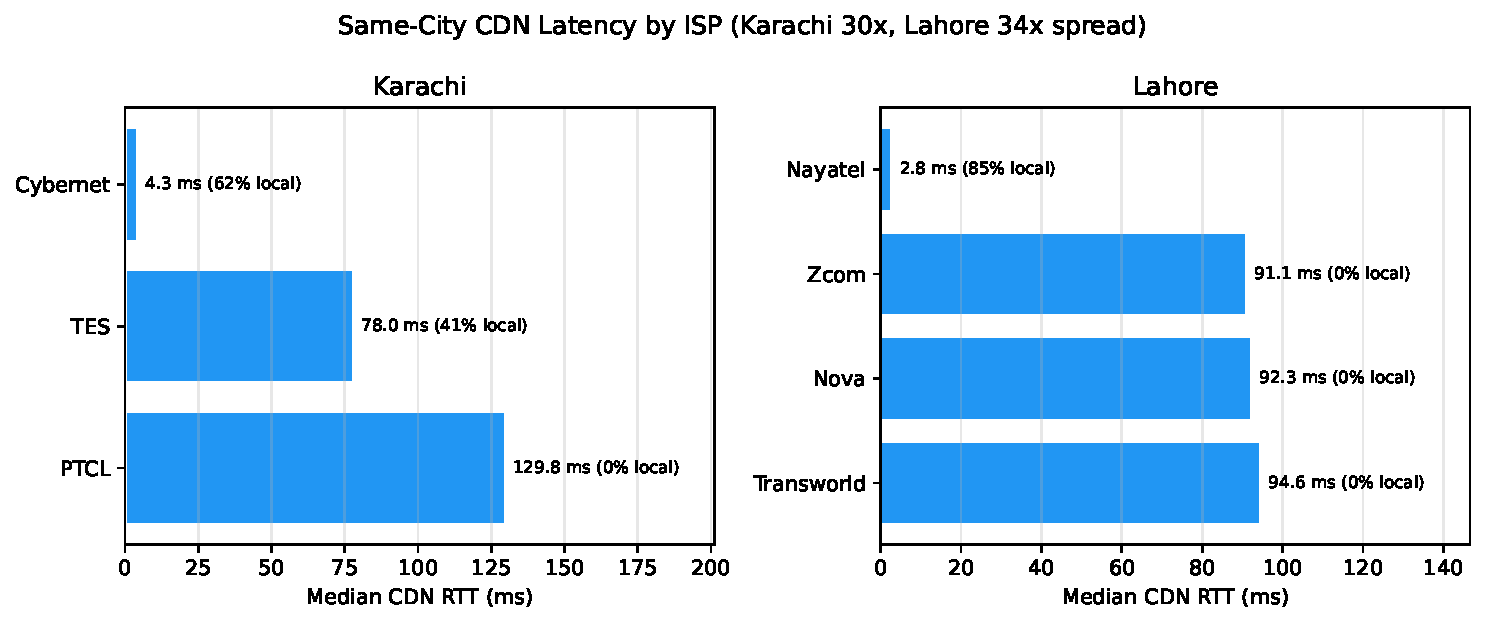
\includegraphics[width=\columnwidth]{fig_rq4_same_city_cdn.pdf}
  \caption{Median CDN latency by ISP, restricted to vantages in the same city. Karachi (Cybernet, TES, PTCL) and Lahore (Nayatel, Nova, Transworld, Zcom) each show a 30$\times$+ spread with distance held constant.}\label{fig:rq4-same-city}\end{figure}

\section{Discussion}
\label{sec:discussion}
The measurement was built to support one argument, and the full week bears it out. The penalty for
reaching domestic content over an international detour is large where it is structural and, as
measured, stable across the day---under 3 percentage points of diurnal variation---so it is not a
capacity problem that more bandwidth would solve but a routing and hosting problem that local
exchange would; % [Correction 13a] "83% flapping pairs also served domestically" softened to 44.8% and reframed as concentrated in a few sites, not a general routing-choice claim.
\hl{and since 44.8\% of the probe--site pairs that ever hairpin are served domestically
on other rounds of the same week, a domestic path demonstrably exists for a meaningful share of
hairpinning traffic, concentrated in a small number of identifiable sites rather than spread
across the sample.}

The exchange is already present in three cities with
dozens of connected members, and its own figures put inter-ISP latency through the exchange one to
two orders of magnitude below the international alternative~\cite{pta2026}. Our own data supply
the same counterfactual without leaning on the exchange's self-reported figures: % [Correction 13b] Flapping-pair count and hairpin RTT updated (193 pairs / ~100ms -> 13 pairs / ~118ms) to match the final detector's sample.
\hl{for the 13
flapping pairs, the local-verdict rounds of the \emph{same} probe--site pair measure the domestic
alternative directly (${\sim}25$\,ms against ${\sim}118$\,ms for the structural hairpins), and}

for persistently hairpinned sites the best RTT observed from any other Pakistani ISP to the same
site bounds what peering could achieve---the frontier construction of \S\ref{sec:ratio}, applied
to domestic content. The gap our measurements expose is therefore not between the status quo and a network that
must be built, but between the status quo and one that must be \emph{used}. In the language of a
three-set framing---networks absent from the exchange, networks present but not exchanging routes,
and networks actively peering---the tromboning we measure is a picture of the first two behaviours
at national scale, and moving networks into the third is a matter of configuration and commercial
willingness rather than construction. The CDN cross-section of \S\ref{sec:prelim-cdn} shows what
moving between sets is worth: the same anycast content is a median $12.7\times$ slower on the
largest operator than on the best-peered network in the same country---and more than $40\times$
slower for the worst quarter of ISP--site pairs---a gap closable by peering rather than by
capacity.

The same structure explains the resilience concern that motivates the study. Because
internationally-routed traffic depends on a small number of submarine cables reached through the three
licensed gateways, a cable fault degrades precisely the traffic that need not have gone abroad,
while traffic hosted and exchanged domestically is untouched. The July~2026 SMW5 fault is a
concrete, measured instance: in companion measurements we ran through the fault window from the
same vantages, international paths showed a 31\% rise in jitter and elevated tail latency (one
site degrading to 646\,ms before recovering) while paths to domestically-hosted content showed
no comparable degradation. A functioning
exchange narrows this exposure directly, by keeping domestic traffic domestic.

Three limitations bound these claims. First, our vantages are fixed-broadband RIPE Atlas probes,
hosted disproportionately by technically engaged users in large cities; the majority of Pakistan's
116 million users reach the internet over mobile networks (Jazz, Zong, Telenor, Ufone), for which
we have no vantage, and mobile-core routing may differ in either direction---the strong per-ISP
heterogeneity we measure among fixed ISPs is itself a warning against extrapolating.
Second, RIPE Atlas measures latency and paths but not traffic
volume, so we quantify the per-path cost of tromboning and not its aggregate economic cost---the
foreign transit purchased and the associated outflow of foreign exchange---which would require
volume data we do not have; we therefore leave a traffic-weighted estimate to future work. Third, a
low traceroute RTT to a CDN edge shows only that the network \emph{edge} is local, not that the
content is served locally, since a request may still be fulfilled from a distant point of presence;
we treat the CDN class accordingly and do not read a local edge as proof of local service.

\section{Conclusion}
Measured from inside the country, Pakistan's internet routing sends a substantial share of domestic
traffic abroad even though a domestic exchange exists to keep it home. Over a week of uniform
measurement from every connected Pakistani vantage to a fixed, reproducibly sampled set of one
hundred sites, classified by an IP-geolocation-independent detector, % [Correction 14] Headline numbers updated for the final detector: 15.1%->5.52% trombone rate, ISP range 3-31%->0.0-11.3%, flapping-domestic-path share 83%->44.8%, trace count 222,944->218,480.
\hl{we find that 5.52\% of traces to
domestically-hosted sites leave the country and return---at 0.0\% from the best-routed ISPs and
11.3\% from the largest; that international paths never exceed ten times the speed-of-light floor
while a quarter of domestic paths do; that the penalty is structural, not diurnal; that the same
CDN content varies by more than an order of magnitude between well-peered and poorly-peered ISPs;
and that 44.8\% of the probe--site pairs that ever hairpin are also served domestically within the
same week, concentrated in a small minority of sites rather than universal across the sample,
while not one of the week's 218,480 traces crossed either of the country's exchange fabrics.}

The remedy is already in place; what our measurements document is the cost of not using it. Beyond this run,
the same framework extends to a longer horizon, to repeated measurement that ranges the tromboning
rate over time, and---by holding a continuous normal-day baseline---to capturing the next cable
fault as a clean before-during-after rather than, as before, against an already-degraded state.

\bibliographystyle{ACM-Reference-Format}
\bibliography{references}


\end{document}
